\documentclass[12pt,letterpaper]{article}

\usepackage{amsmath, amsthm}
\usepackage{microtype, parskip}
\usepackage[comma,numbers,sort&compress]{natbib}
\usepackage{lineno}
\usepackage{docmute}
\usepackage{caption, subcaption, multirow, morefloats, rotating}
\usepackage{wrapfig}

\frenchspacing

\begin{document}

\section*{Results}

The results of the analyses described above take one of two forms: direct inspection of parameter posterior estimates from both models, and downstream estimates of diversity and diversification rates based on posterior predictive simulations from the birth-death model because this model has a better fit to the observed occurrence information.

\subsection*{Comparing parameter estimates from the pure-presence and birth-death models}

% look at the posterior predictive checks
%   which model has better fit
%   what does that mean?


\begin{figure}[ht]
  \begin{subfigure}[b]{0.45\textwidth}
    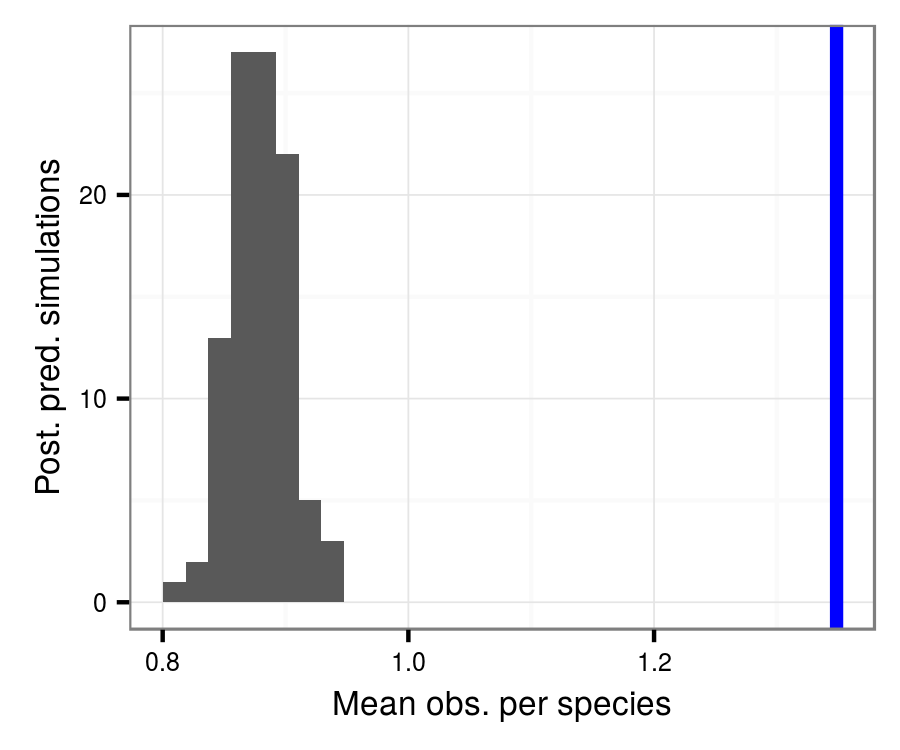
\includegraphics[width=\textwidth,height=0.3\textheight,keepaspectratio=true]{figure/pred_occ}
    \caption{Pure-presence model}
    \label{fig:ppc_pure_presence}
  \end{subfigure}
  \begin{subfigure}[b]{0.45\textwidth}
    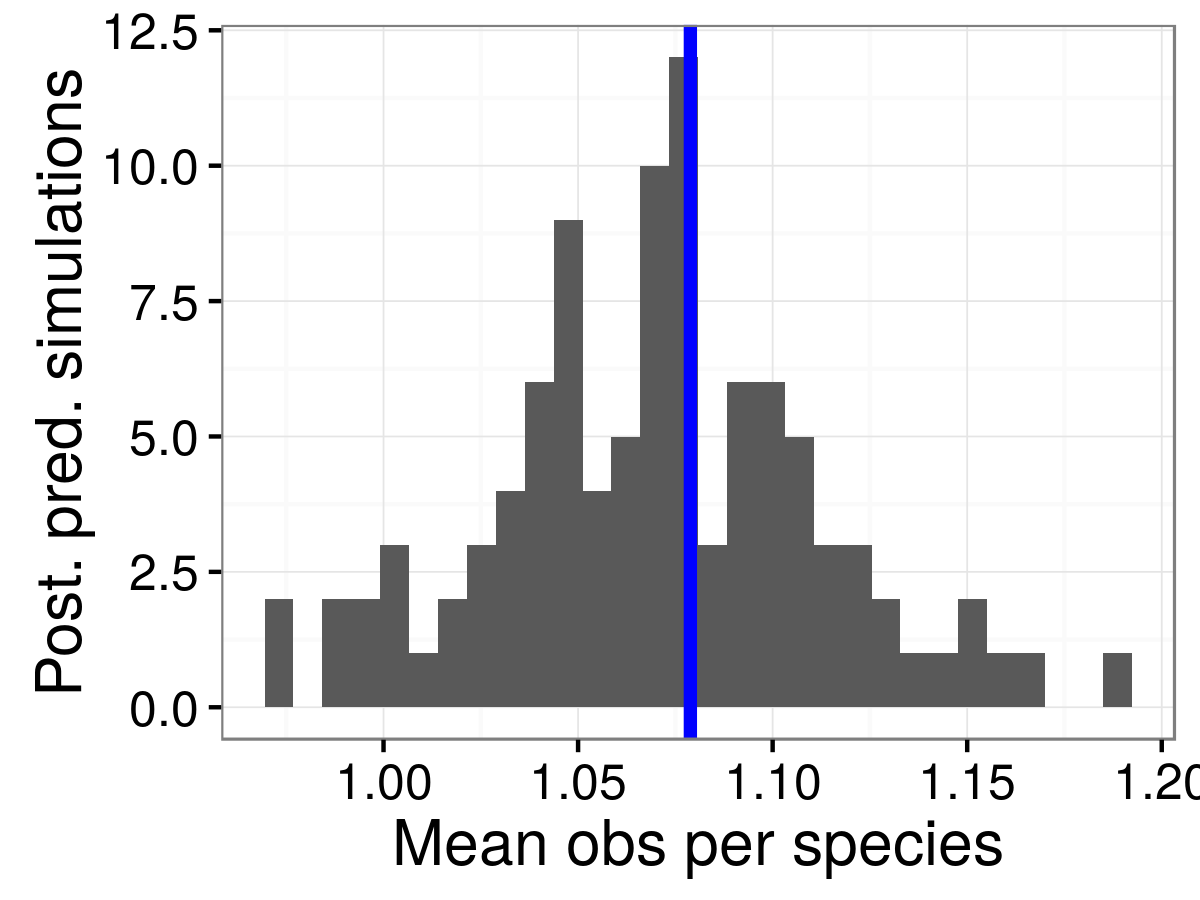
\includegraphics[width=\textwidth,height=0.3\textheight,keepaspectratio=true]{figure/pred_occ_bd}
    \caption{Birth-death model}
    \label{fig:ppc_birth_death}
  \end{subfigure}
  \caption[Posterior predictive check of average occurrence]{Comparison of the average observed number of occurrences per species (blue line) to the average number of occurrences from 100 posterior predictive datasets using the posterior estimates from the pure-presence and birth-death models.}
  \label{fig:ppc}
\end{figure}

Comparison of the posterior predictive results from the pure-presence and birth-death models reveals a striking difference in performance of either model to predict the structure of the underlying data (Fig. \ref{fig:ppc}). The simulated datasets generated from the birth-death model are clearly able to better reproduce the observed average number of occurrence than the pure-presence model which underestimates the observed average number of occurrences. This result means that inferences based on the birth-death model are more likely to be representative of the underlying data than inferences based on the pure-presence model. Further inspection of the posterior parameter estimates from both models gives further insight into the resins for this difference in posterior predictive results \citep{Gelman2013d}. 

Increases in the occurrence probability of an ecotype is interpreted as an increase in the commonness of that ecotype in the species pool. In turn, decreases in the occurrence probability of an ecotype are interpreted to a decrease in the commonness of that ecotype in the species pool. Additionally, when the uncertainty surrounding a probability estimate is very high, as with arboreal insectivores, this is interpreted as complete separation which means that that ecotype has most likely all but disappeared from the species pool \citep{Gelman2007}. In logistic regression, high uncertainty in the estimates of the underlying log-odds of occurrence, origination, or survival tends to indicate extreme rarity or complete absence of the specific ecotype. The latter is called complete separation and occurs when there is no uncertainty in the effect of a covariate on presence/absence. The problem of complete separation is mitigated by the hierarchical modeling strategy used here \citep{Gelman2013d,Gelman2007,McElreath2016}.

Estimates of occurrence probability estimated from the pure-presence model and estimates of origination probability from the birth-death model are broadly similar (Fig. \ref{fig:eco_occur}), \ref{fig:eco_origin}); this is not the case for the survival probability estimates (Fig. \ref{fig:eco_survival}). This result supports the idea that changes to the North American regional species pool is more likely due to changes in origination than extinction, a result to which I will return to later in the discussion of per-capita diversification, origination, and extinction rates. For most ecotypes, occurrence and origination probability estimates increase with time (Fig. \ref{fig:eco_origin}). This makes sense given that, over time, all species that have at least one observed occurrence must have had that occurrence by the last time point, so our certainty in a species occurring must increase with time. Notably, ecotypes with arboreal components do not appear to follow the same pattern as most other ecotypes; instead, origination probabilities appear relatively flat with high posterior variance for most of the Cenozoic. For most ecotypes, occurrence or origination probability is estimated with less uncertainty than its estimate of survival probability (Fig. \ref{fig:eco_occur}, \ref{fig:eco_origin}, \ref{fig:eco_survival}). 



\begin{figure}[ht]
  \centering
  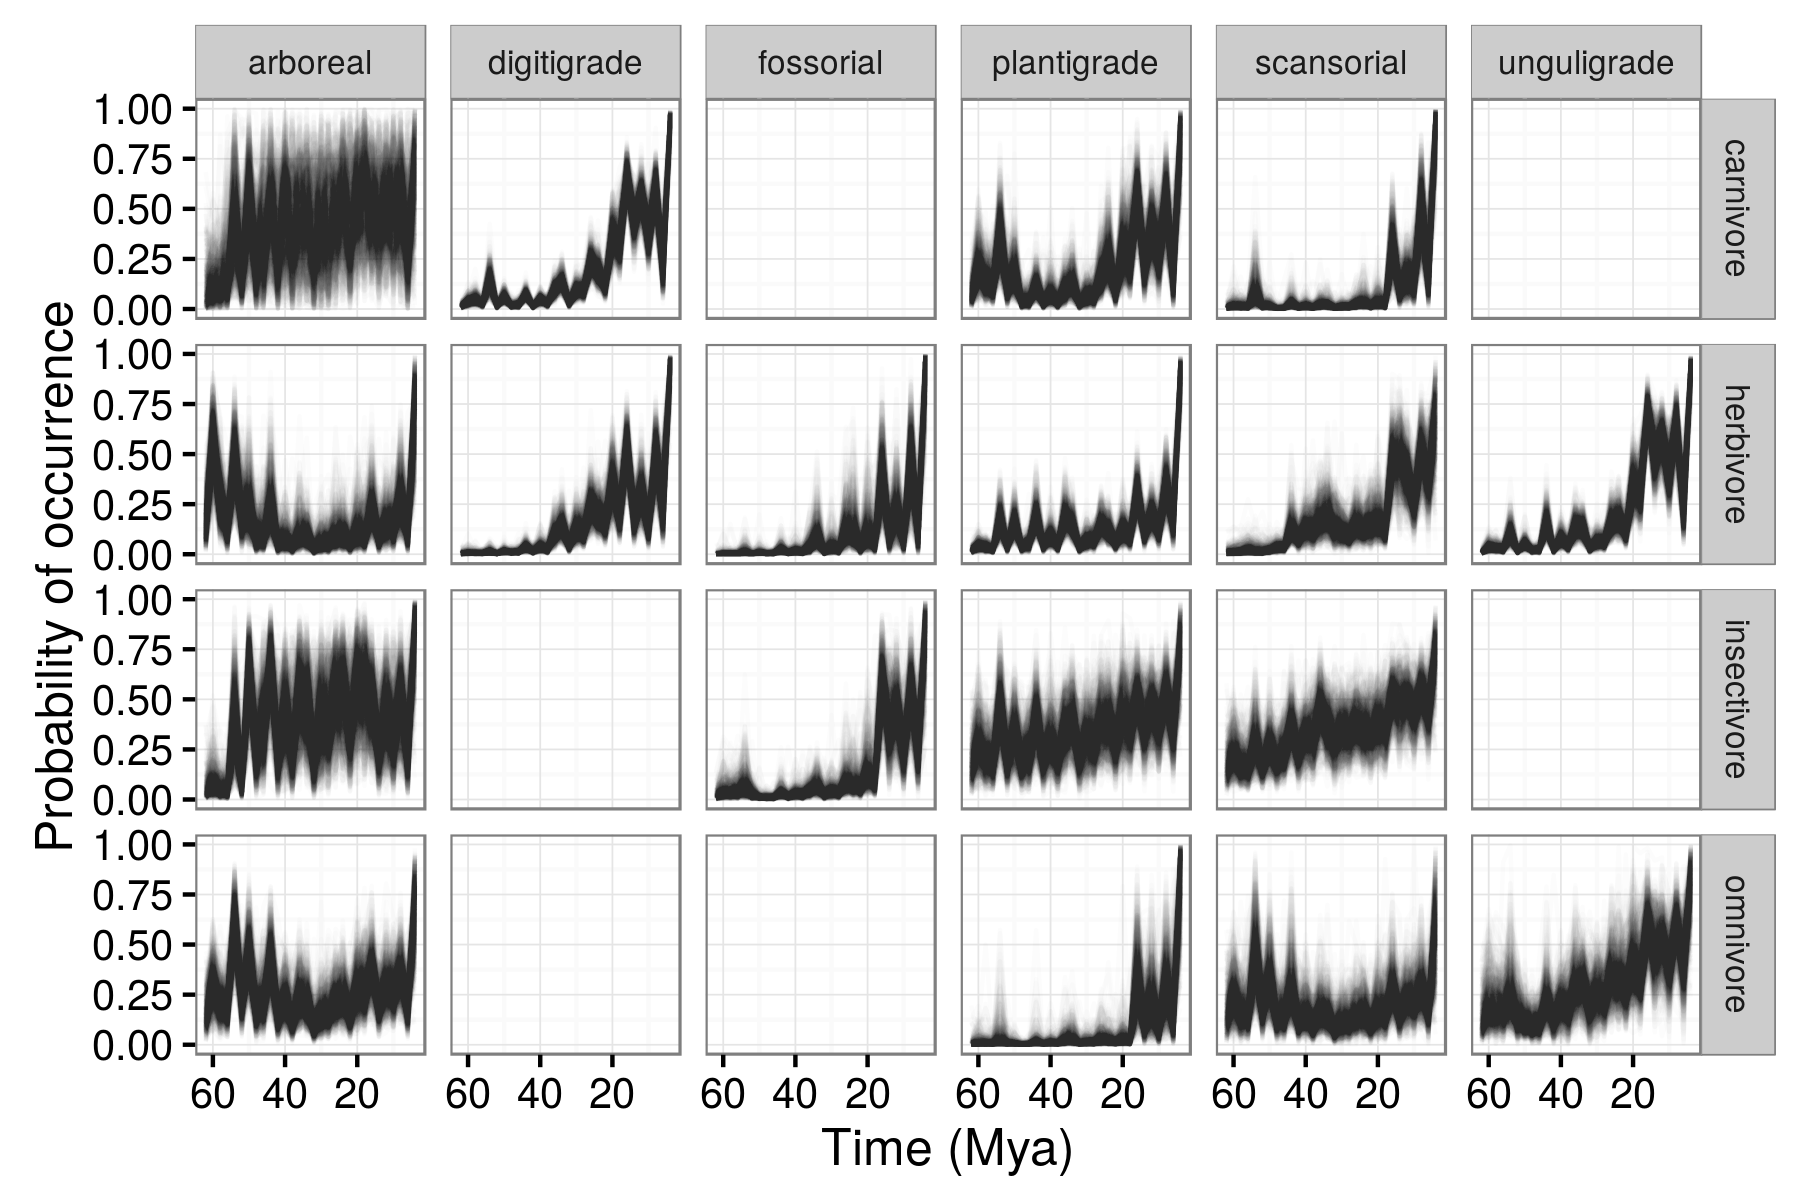
\includegraphics[width=\textwidth,height=0.4\textheight,keepaspectratio=true]{figure/ecotype_occurrence}
  \caption[Ecotype occurrence probability estimated from the pure-presence model]{Probability of a mammal ecotype occurring over time as estimated from the pure-presence model. Each panel depicts 100 random samples from the model's posterior. The columns are by locomotor category and rows by dietary category; their intersections are the observed and analyzed ecotypes. Panels with no lines are ecotypes not observed in the dataset.}
  \label{fig:eco_occur}
\end{figure}

\begin{figure}[ht]
  \centering
  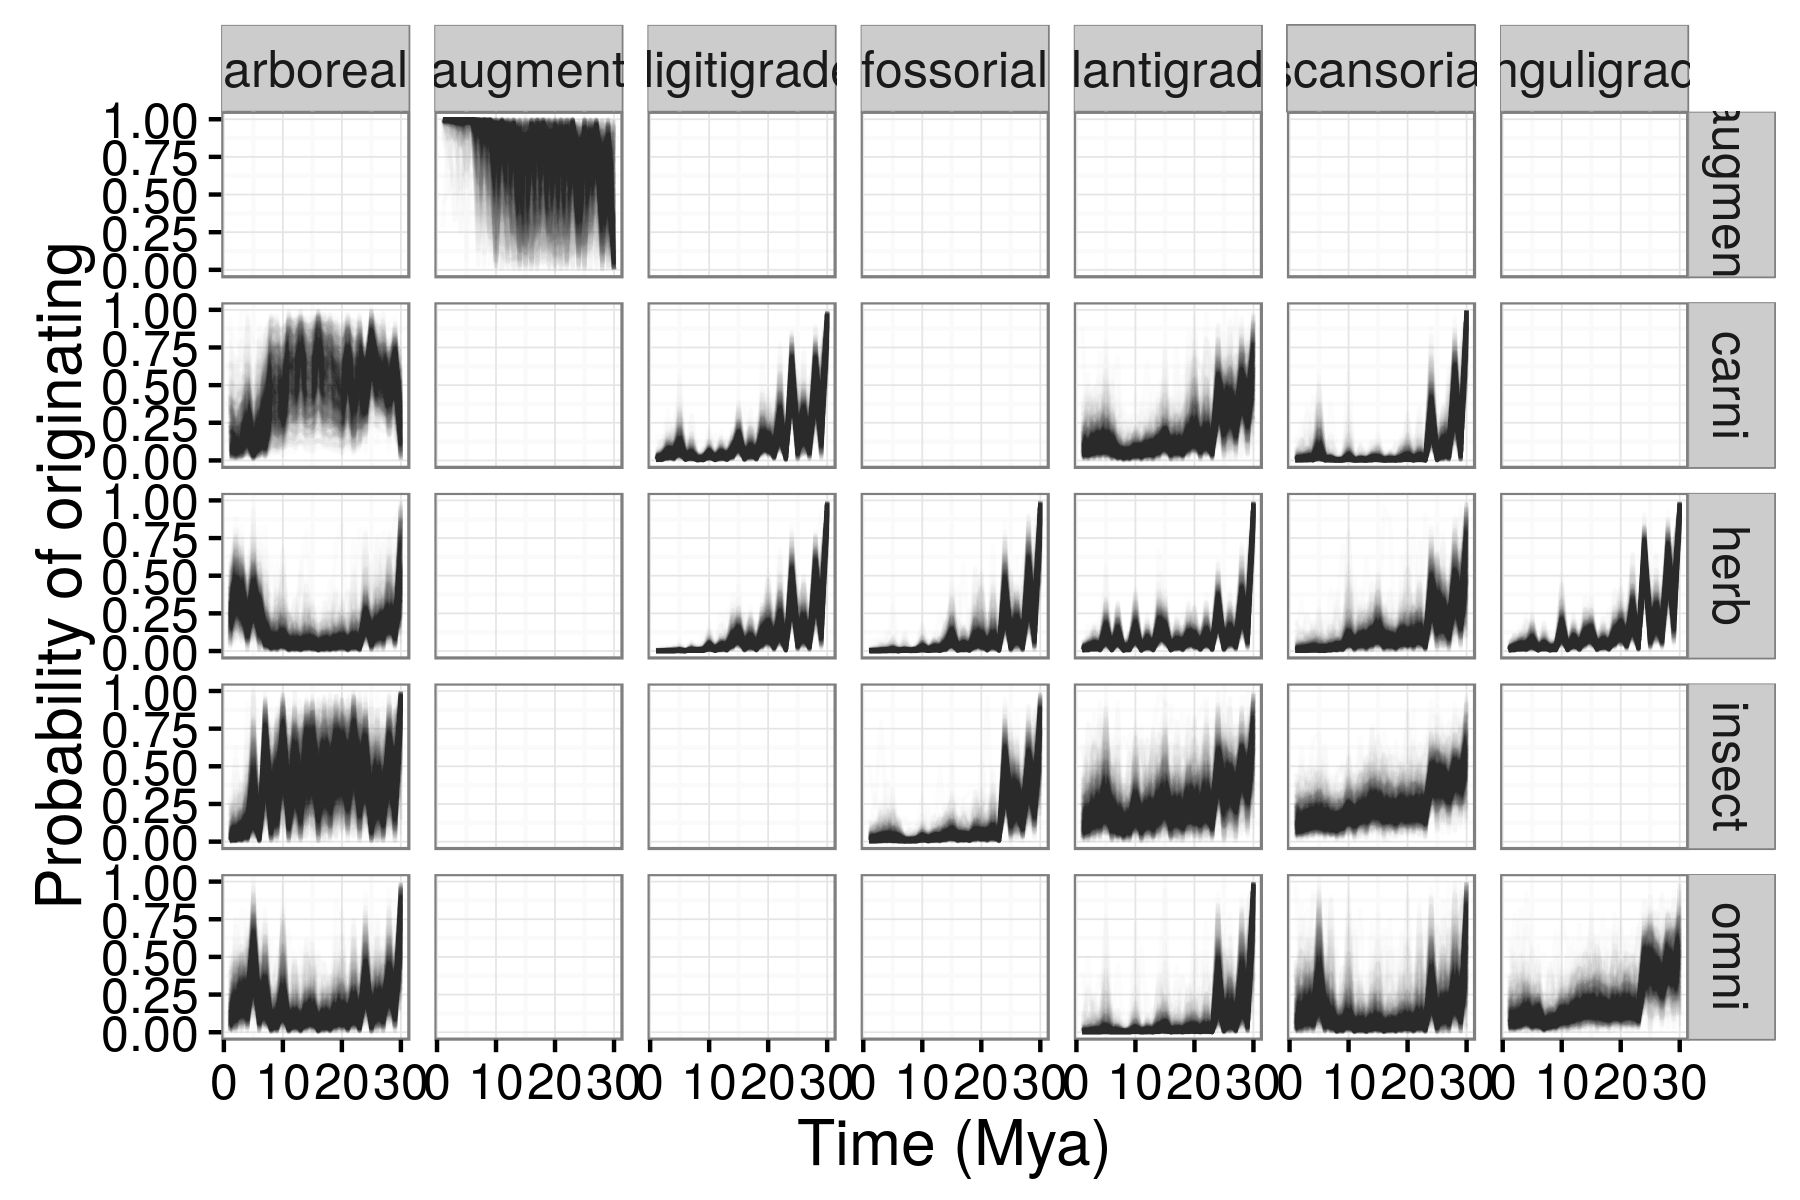
\includegraphics[width=\textwidth,height=0.4\textheight,keepaspectratio=true]{figure/ecotype_origin_bd}
  \caption[Ecotype origination probability estimated from the birth-death model]{Probability of a mammal ecotype origination probabliities at each time point as estimated from the birth-death model. Each panel depicts 100 random samples from the model's posterior. The columns are by locomotor category and rows by dietary category; their intersections are the observed and analyzed ecotypes. Panels with no lines are ecotypes not observed in the dataset.}
  \label{fig:eco_origin}
\end{figure}

\begin{figure}[ht]
  \centering
  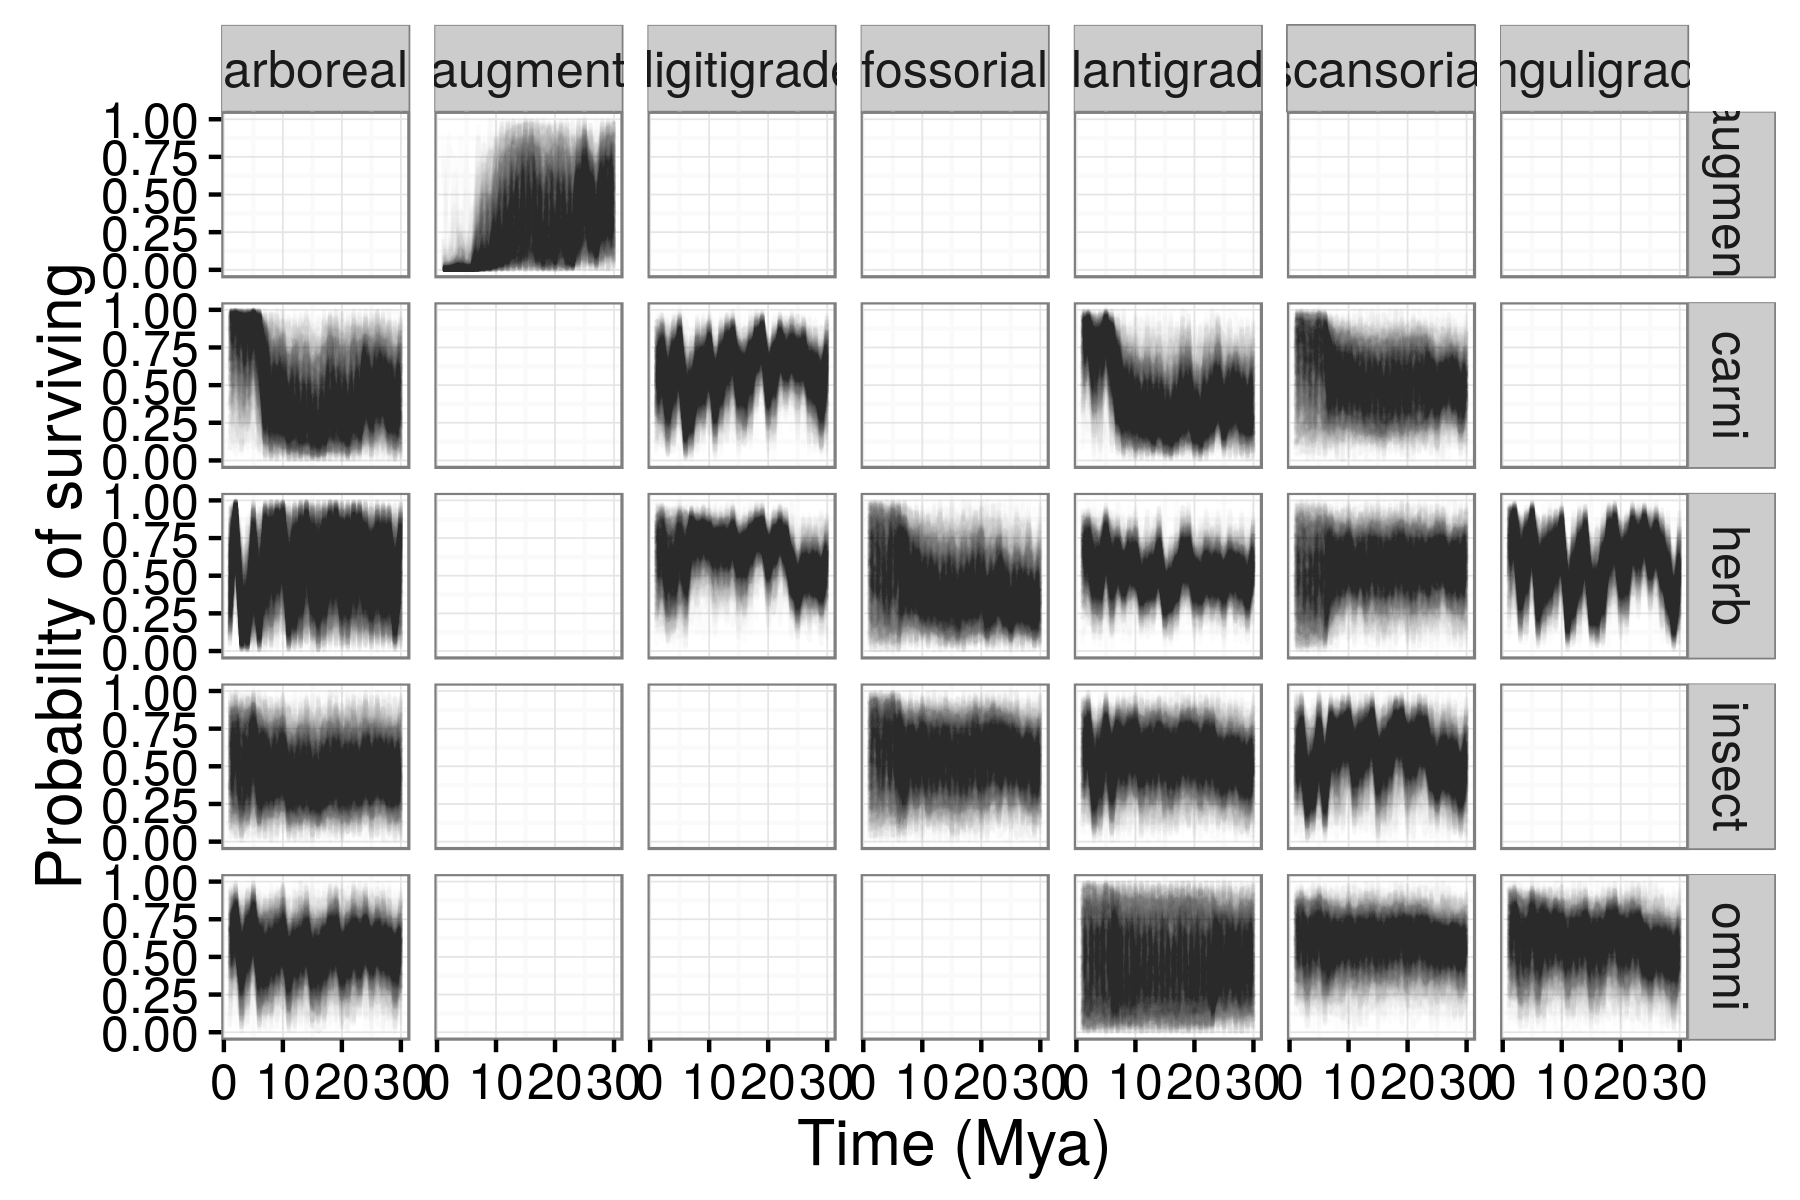
\includegraphics[width=\textwidth,height=0.4\textheight,keepaspectratio=true]{figure/ecotype_survival_bd}
  \caption[Ecotype survival probability estimated from the birth-death model]{Probability of a mammal ecotype survival probabilities at each time point as estimated from the birth-death model. Each panel depicts 100 random samples from the model's posterior. The columns are by locomotor category and rows by dietary category; their intersections are the observed and analyzed ecotypes. Panels with no lines are ecotypes not observed in the dataset.}
  \label{fig:eco_survival}
\end{figure}


The pure-presence and birth-death models have similar estimates of the relationship between species mass and the probability of sampling a species that is present (Fig. \ref{fig:mass_preserve}). For both models this relationship is at least weakly positive, which means that as species body mass increases it is expected that they are more likely to be sampled if present. The estimated relationship from the pure-presence model is with greater uncertainty than that from the birth-death model (Fig. \ref{fig:mass_preserve}). These results are consistent with the intuition that larger fossils are easier to sample because they are more visible to the eye. In turn, this means that observed occurrence histories small bodied species are more likely to have gaps, where \(y = 0\) for that species the true state \(z\) is 1. 

\begin{figure}[ht]
  \begin{subfigure}[b]{0.45\textwidth}
    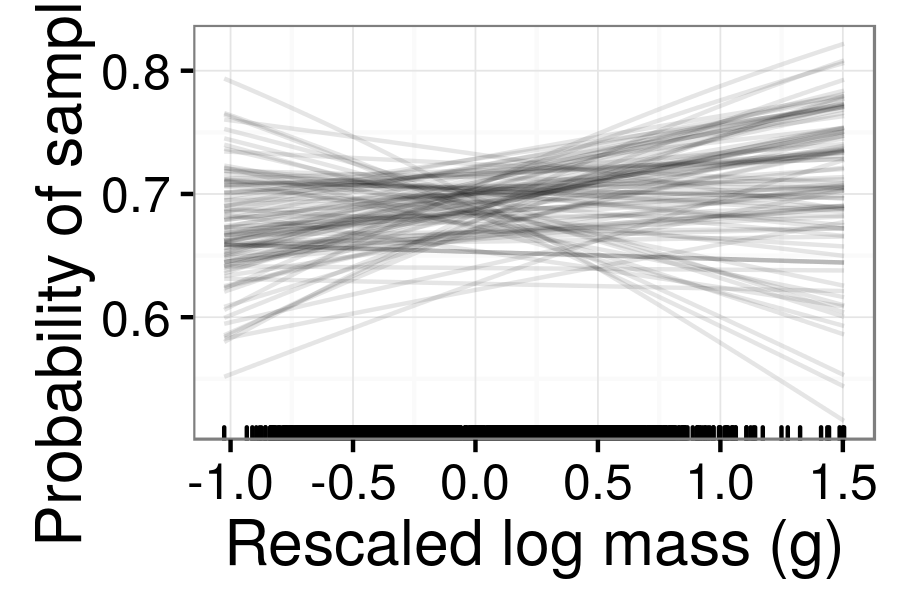
\includegraphics[width=\textwidth,height=0.4\textheight,keepaspectratio=true]{figure/mass_on_samp}
    \caption{Pure-presence model}
    \label{fig:mass_preserve_pure_pres}
  \end{subfigure}
  \begin{subfigure}[b]{0.45\textwidth}
    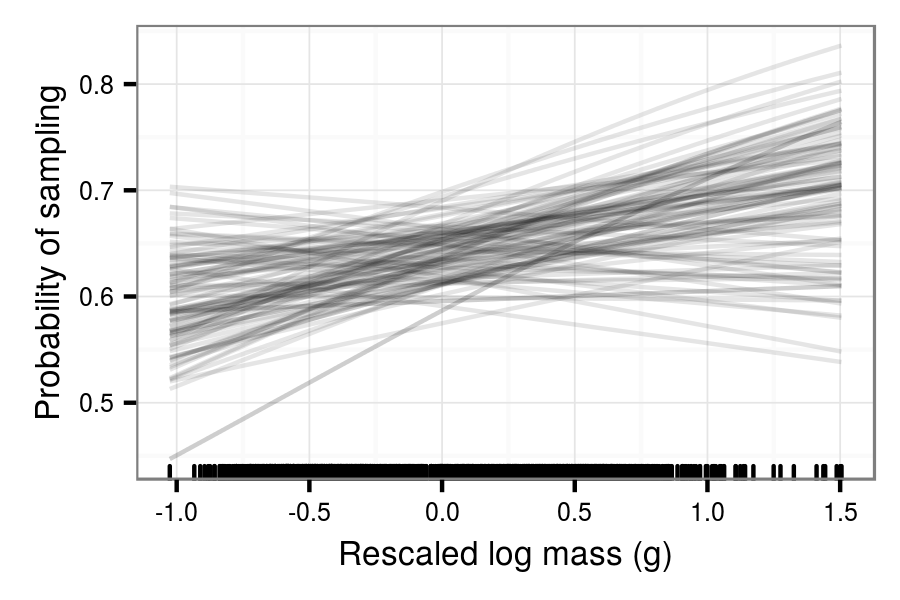
\includegraphics[width=\textwidth,height=0.4\textheight,keepaspectratio=true]{figure/mass_on_samp_bd}
    \caption{Birth-death model}
    \label{fig:mass_preserve_bd}
  \end{subfigure}
  \caption[Estimates of the effect of mass on observation probability]{Estimates of the effect of species mass on probability of sampling a present species (\(p\)). Mass has been log-transformed, centered, and rescaled; this means that a mass of 0 corresponds to the mean of log-mass of all observed species and that mass is in standard deviation units. Estimates are from both the pure-presence and birth-death models.}
  \label{fig:mass_preserve}
\end{figure}

%For the pure-presence model, species mass is found to have either no relationship with occurrence or a negative one (Fig. \ref{fig:mass_occur}). A negative relationship between body size and occurrence is interpreted to mean that large bodied species are likely to occur less frequently than smaller bodied species. Note that all variation in estimates between ecotypes (Fig. \ref{fig:mass_occur}) is due to differences in ecotype-specific occurrence probability and the associated effects of plant phase; the effect of mass was considered constant for all ecotypes.

There is broad congruence between the estimated effect of body mass on occurrence proability (Fig. \ref{fig:mass_occur}) and the effect of species mass on body mass on origination probaiblity (Fig. \ref{fig:mass_origin}). The striking pattern is higher probability of origination for species with body sizes closer to the mean than either extremes. This result is consistent with the canonically normal distribution of mammal body sizes \citep{Smith2004}; it is then expected that the most likely to occur species would be those from the middle of the distribution, and that species originating will on average be of average mass, especially considering species shared common ancestry \citep{Felsenstein1985b}. All variation in estimates between ecotypes (Fig. \ref{fig:mass_occur}, \ref{fig:mass_origin}) is due to differences in ecotype-specific origination probabilities and the associated effects of plant phase; the effect of mass was considered constant for all ecotypes.

\begin{figure}[ht]
  \centering
  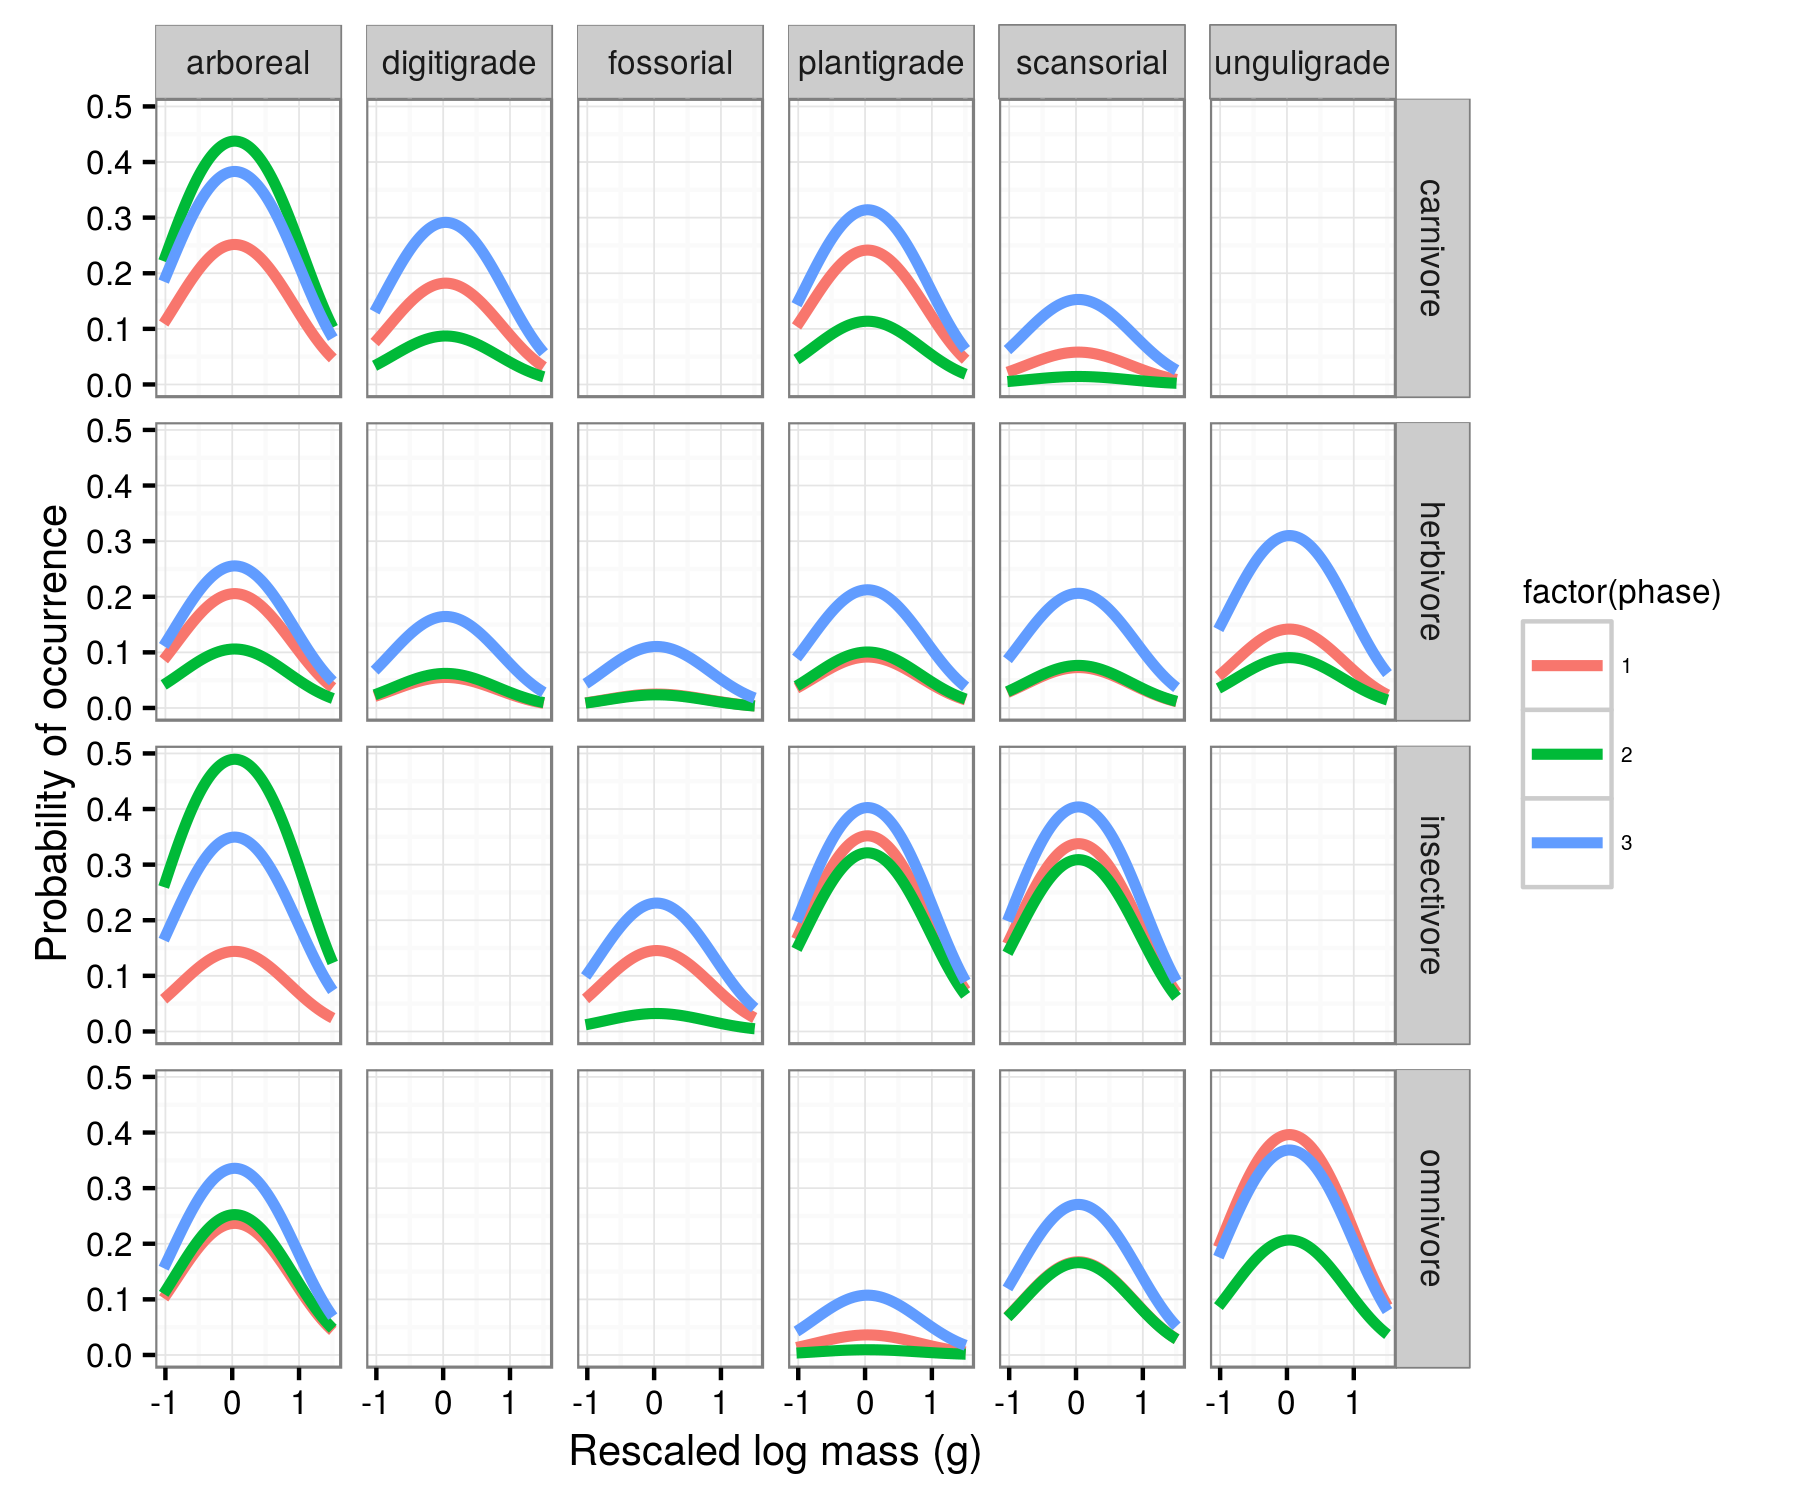
\includegraphics[width=\textwidth,height=0.4\textheight,keepaspectratio=true]{figure/mass_on_pres}
  \caption[Effect of mass on probability of species occurrence as estimated from the pure-presence model]{Mean estimate of the effect of species mass on the probability of a species occurrence for each of the three plant phases. The effect of mass is considered constant over time and that the only aspect of the model that changes with plant phase is the intercept of the relationship between mass and occurrence. The three plant phases are indicated by the color of the line. Mass has been log-transformed, centered, and rescaled; this means that a mass of 0 corresponds to the mean of log-mass of all observed species and that mass is in standard deviation units. For clarity, only the mean estimates of the effects of mass and plant phase are plotted.}
  \label{fig:mass_occur}
\end{figure}

\begin{figure}[ht]
  \centering
  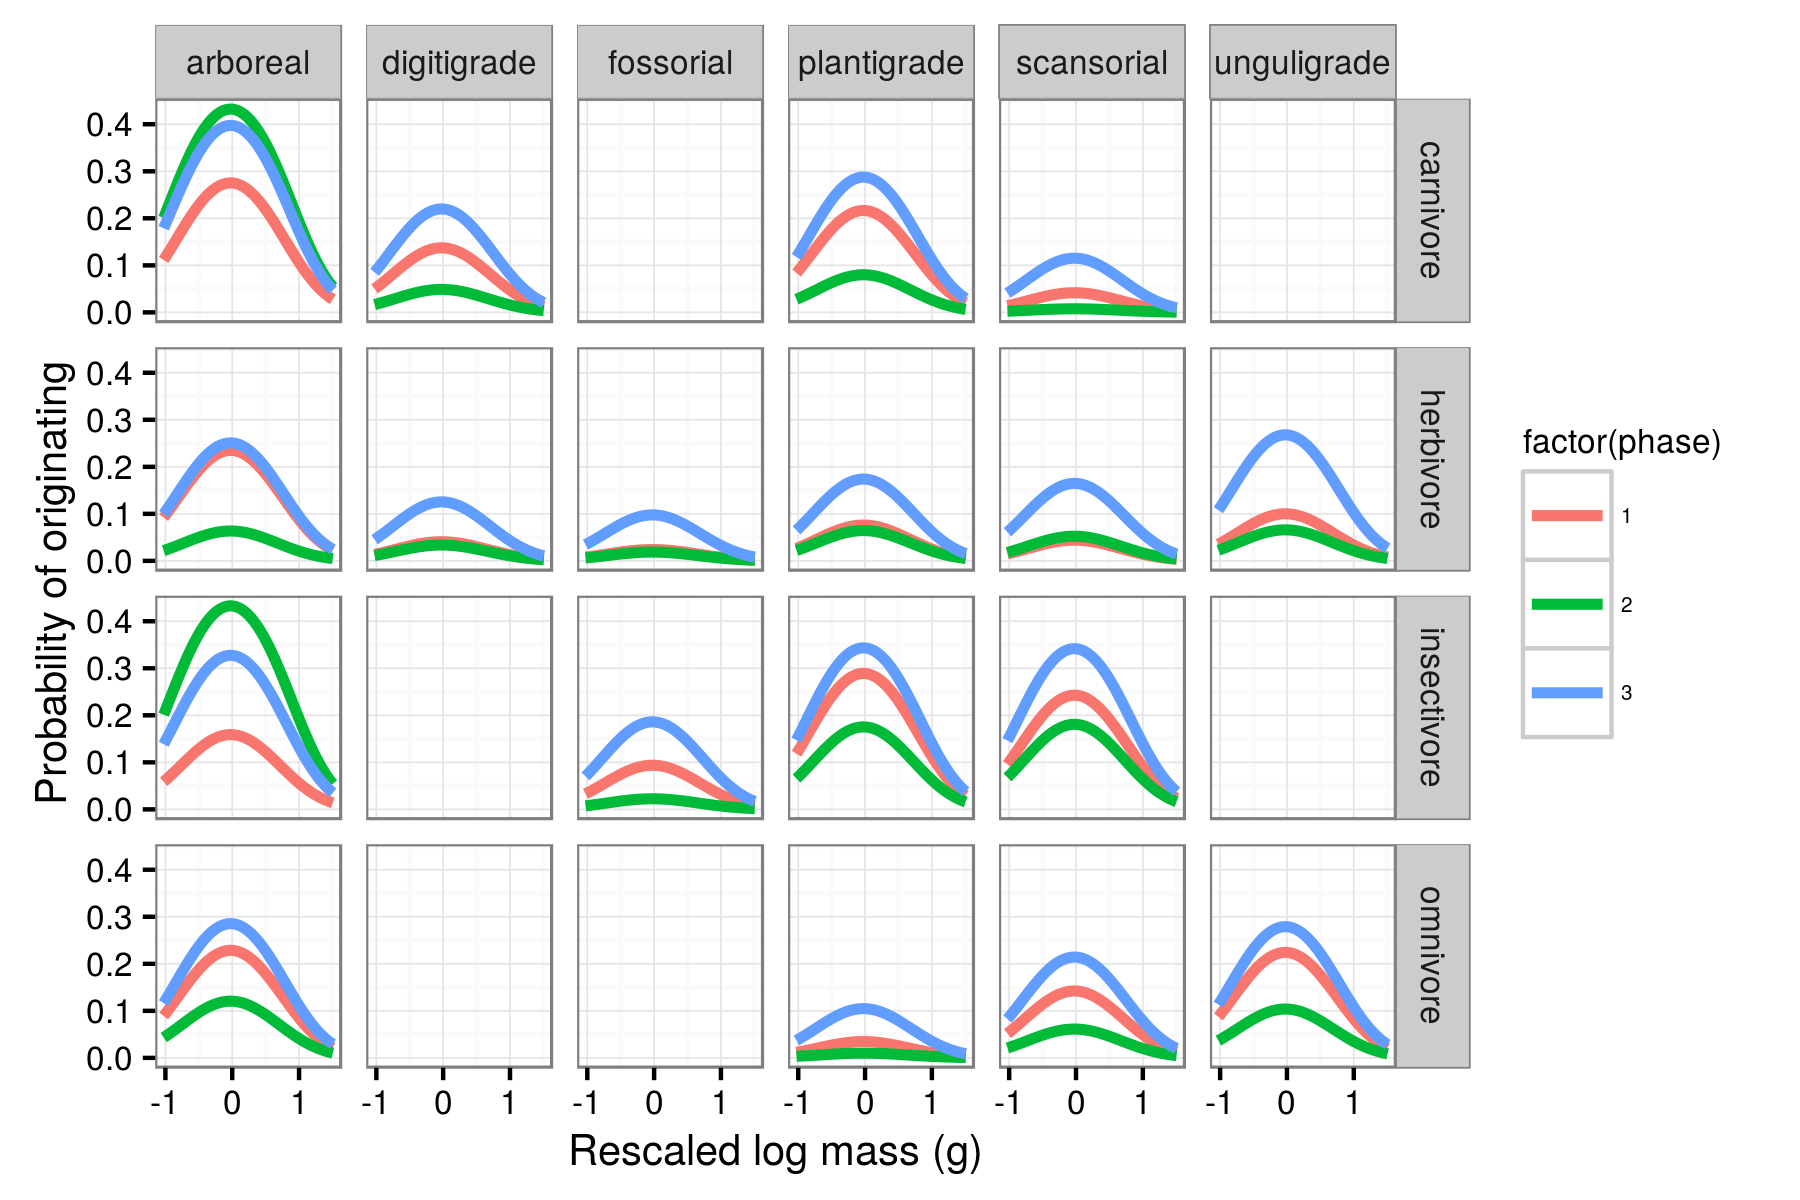
\includegraphics[width=\textwidth,height=0.4\textheight,keepaspectratio=true]{figure/mass_on_origin_bd}
  \caption[Effect of mass on probability of species origination as estimated from the birth-death model]{Mean estimate of the effect of species mass on the probability of a species originating for each of the three plant phases. The effect of mass is considered constant over time and that the only aspect of the model that changes with plant phase is the intercept of the relationship between mass and origination. The three plant phases are indicated by the color of the line. Mass has been log-transformed, centered, and rescaled; this means that a mass of 0 corresponds to the mean of log-mass of all observed species and that mass is in standard deviation units. For clarity, only the mean estimates of the effects of mass and plant phase are plotted.}
  \label{fig:mass_origin}
\end{figure}

In contrast, the effect of species mass on probability of survival as estimated from the birth-death model (Fig. \ref{fig:mass_survival}) is consistent with previous findings that there is little effect of mass on extinction for North American mammals for the Cenozoic \citep{Smits2015b,Tomiya2013}. Note that all variation between ecotypes depicted in Figure \ref{fig:mass_survival} is due to differences in ecotype-specific survival probability and the associated effects of plant phase; the effect of mass was considered constant for all ecotypes (Eqs. \ref{eq:pure_presence}, \ref{eq:birth_death}).

\begin{figure}[ht]
  \centering
  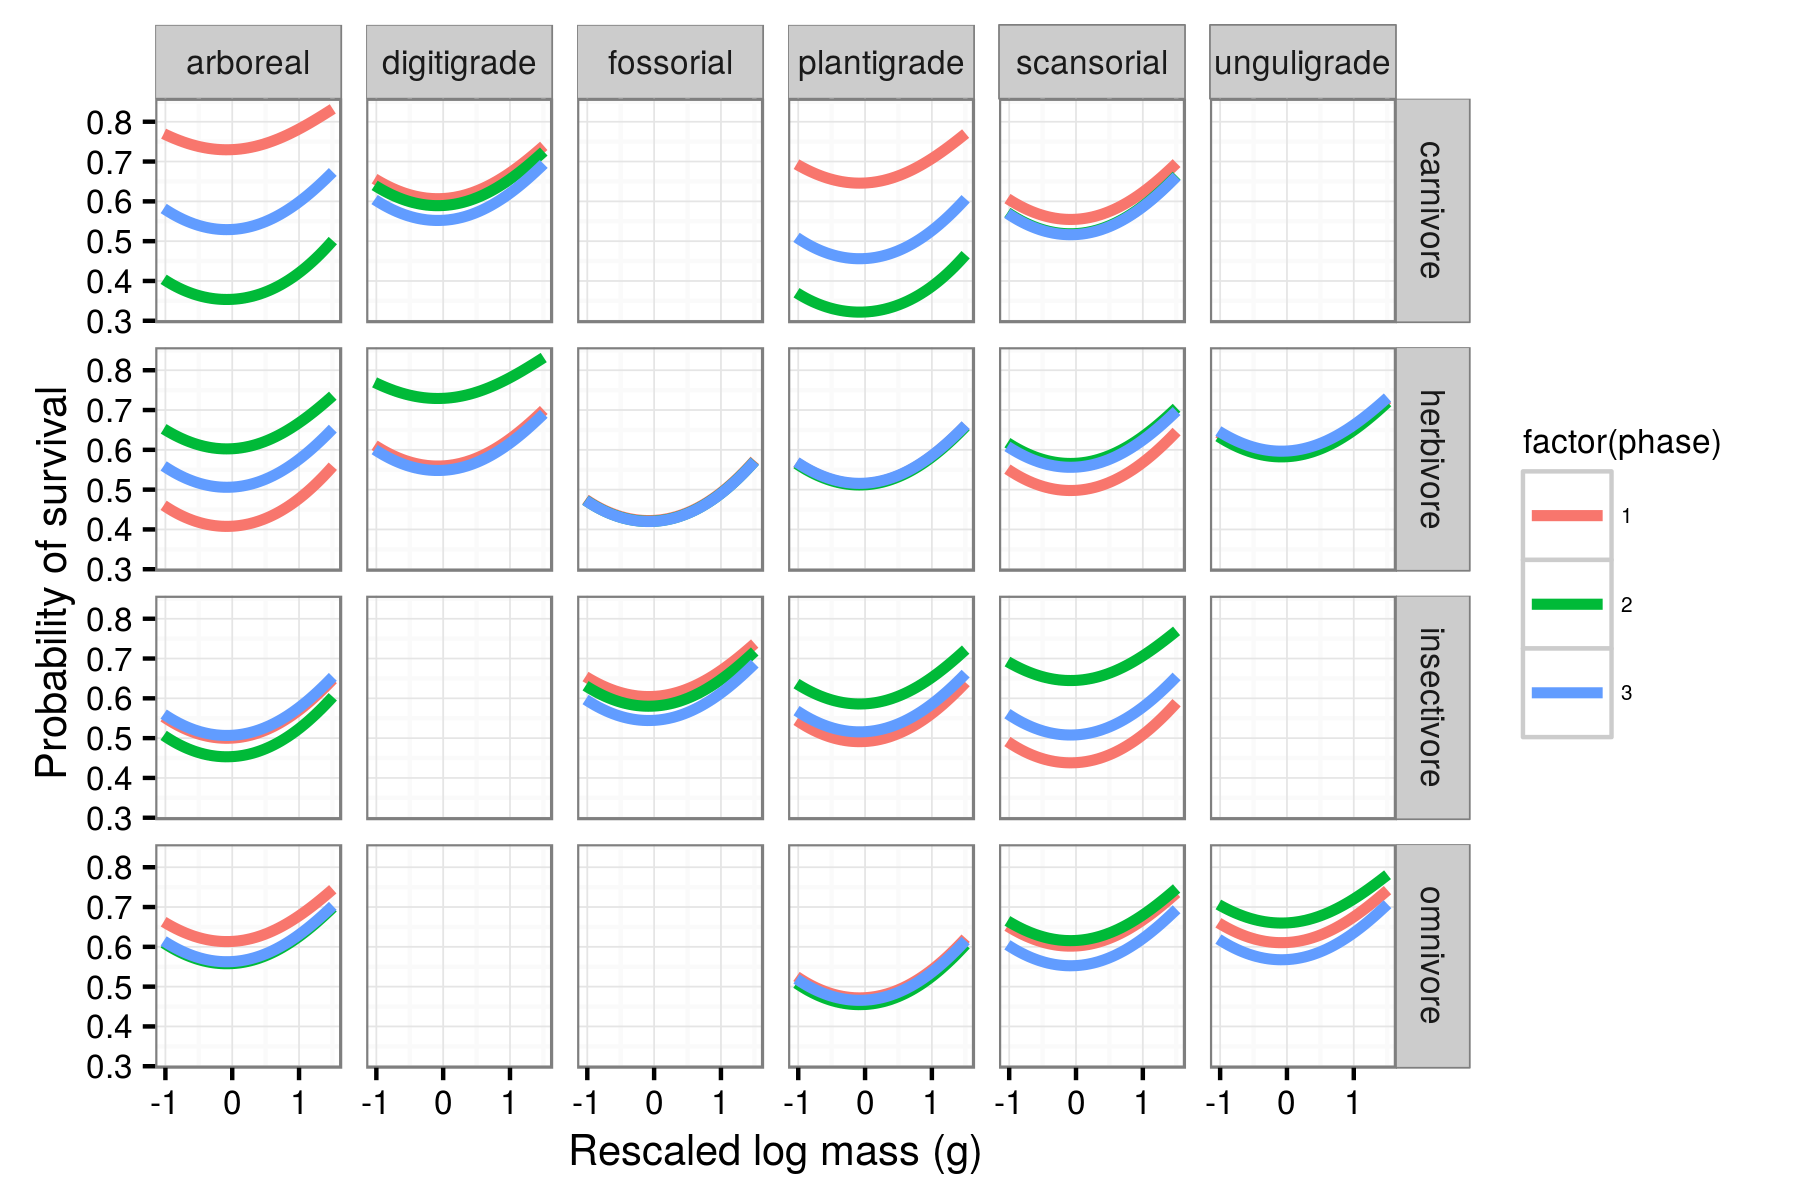
\includegraphics[width=\textwidth,height=0.4\textheight,keepaspectratio=true]{figure/mass_on_surv_bd}
  \caption[Effect of mass on probability of species survival as estimated from the birth-death model]{Mean estimate of the effect of species mass on the probability of a species survival for each of the three plant phases. The effect of mass is considered constant over time and that the only aspect of the model that changes with plant phase is the intercept of the relationship between mass and survival. The three plant phases are indicated by the color of the line. Mass has been log-transformed, centered, and rescaled; this means that a mass of 0 corresponds to the mean of log-mass of all observed species and that mass is in standard deviation units. For clarity, only the mean estimates of the effects of mass and plant plant are plotted.}
  \label{fig:mass_survival}
\end{figure}


Similarities in parameter estimates between ecotypes may be due to a similar response to environmental factors (Fig. \ref{fig:group_pure_presence}, \ref{fig:group_origin_bd}, and \ref{fig:group_surv_bd}). The estimated group-level effects on ecotype occurrence, origination, or survival are all very different from each other. At best, the effects of temperature on occurrence and origination can be considered congruent (Fig. \ref{fig:group_pure_presence}, \ref{fig:group_origin_bd}). As demonstrated in the comparisons of the effect of body mass on occurrence from the pure-presence model (Fig. \ref{fig:mass_occur}) with the effect of body mass on origination and survival from the birth-death model (Fig. \ref{fig:mass_origin}, and \ref{fig:mass_survival}), there is considerable variation in the effect of plant phases on ecotype-specific estimates.


\begin{figure}[ht]
  \centering
  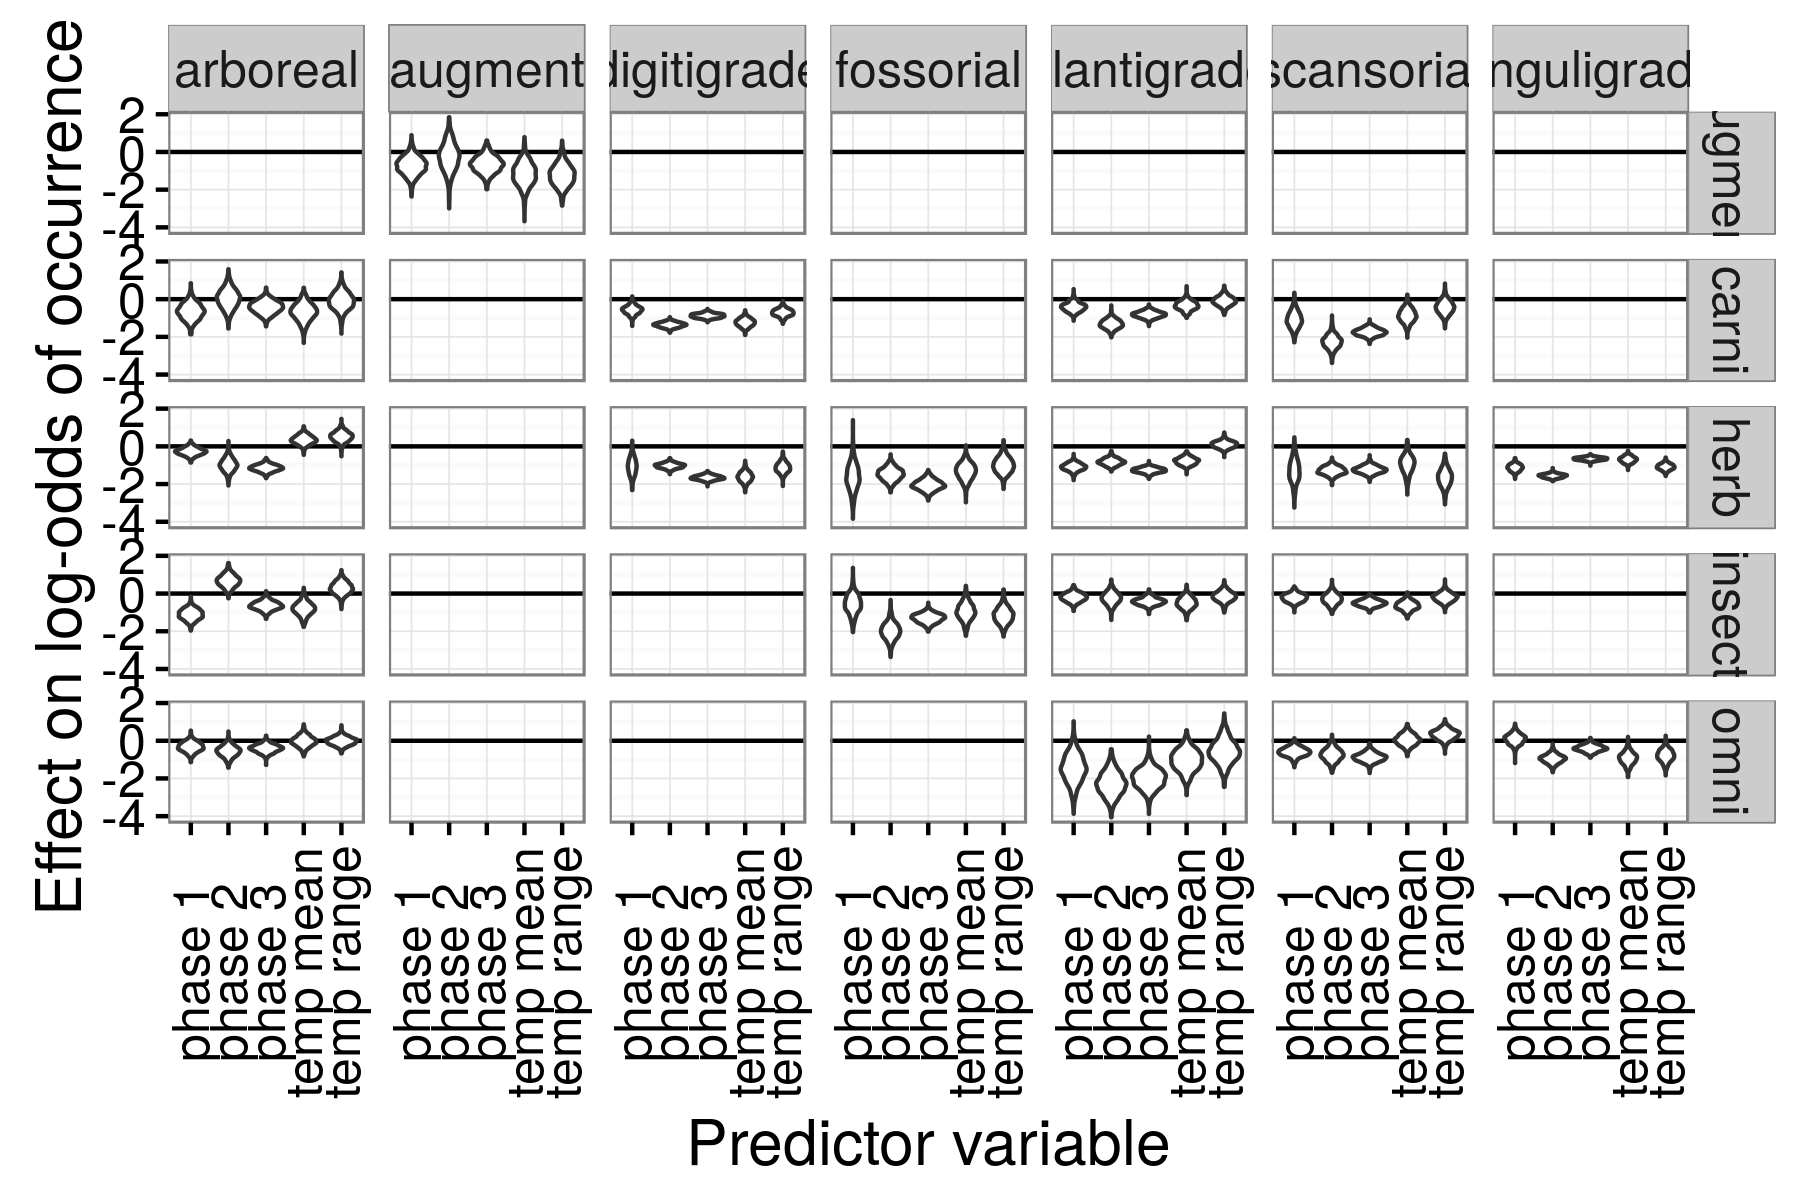
\includegraphics[width=\textwidth,height=0.4\textheight,keepaspectratio=true]{figure/group_on_ecotype}
  \caption[Effects of group-level covariates on log-odds of ecotype occurrence as estimated from the pure-presence model]{Estimated effects of the group-level covariates describing environmental context on log-odds of species occurrence. These estimates are from the pure-presence model. What is plotted is a violin of the distribution of 1000 samples from the approximate posterior. The effect of plant phase graphed here is calculated as Phase 1\( = \gamma_{phase\ 1}\), Phase 2\( = \gamma_{phase\ 1} + \gamma_{phase\ 2}\), and so on.} 
  \label{fig:group_pure_presence}
\end{figure}

\begin{figure}[ht]
  \centering
  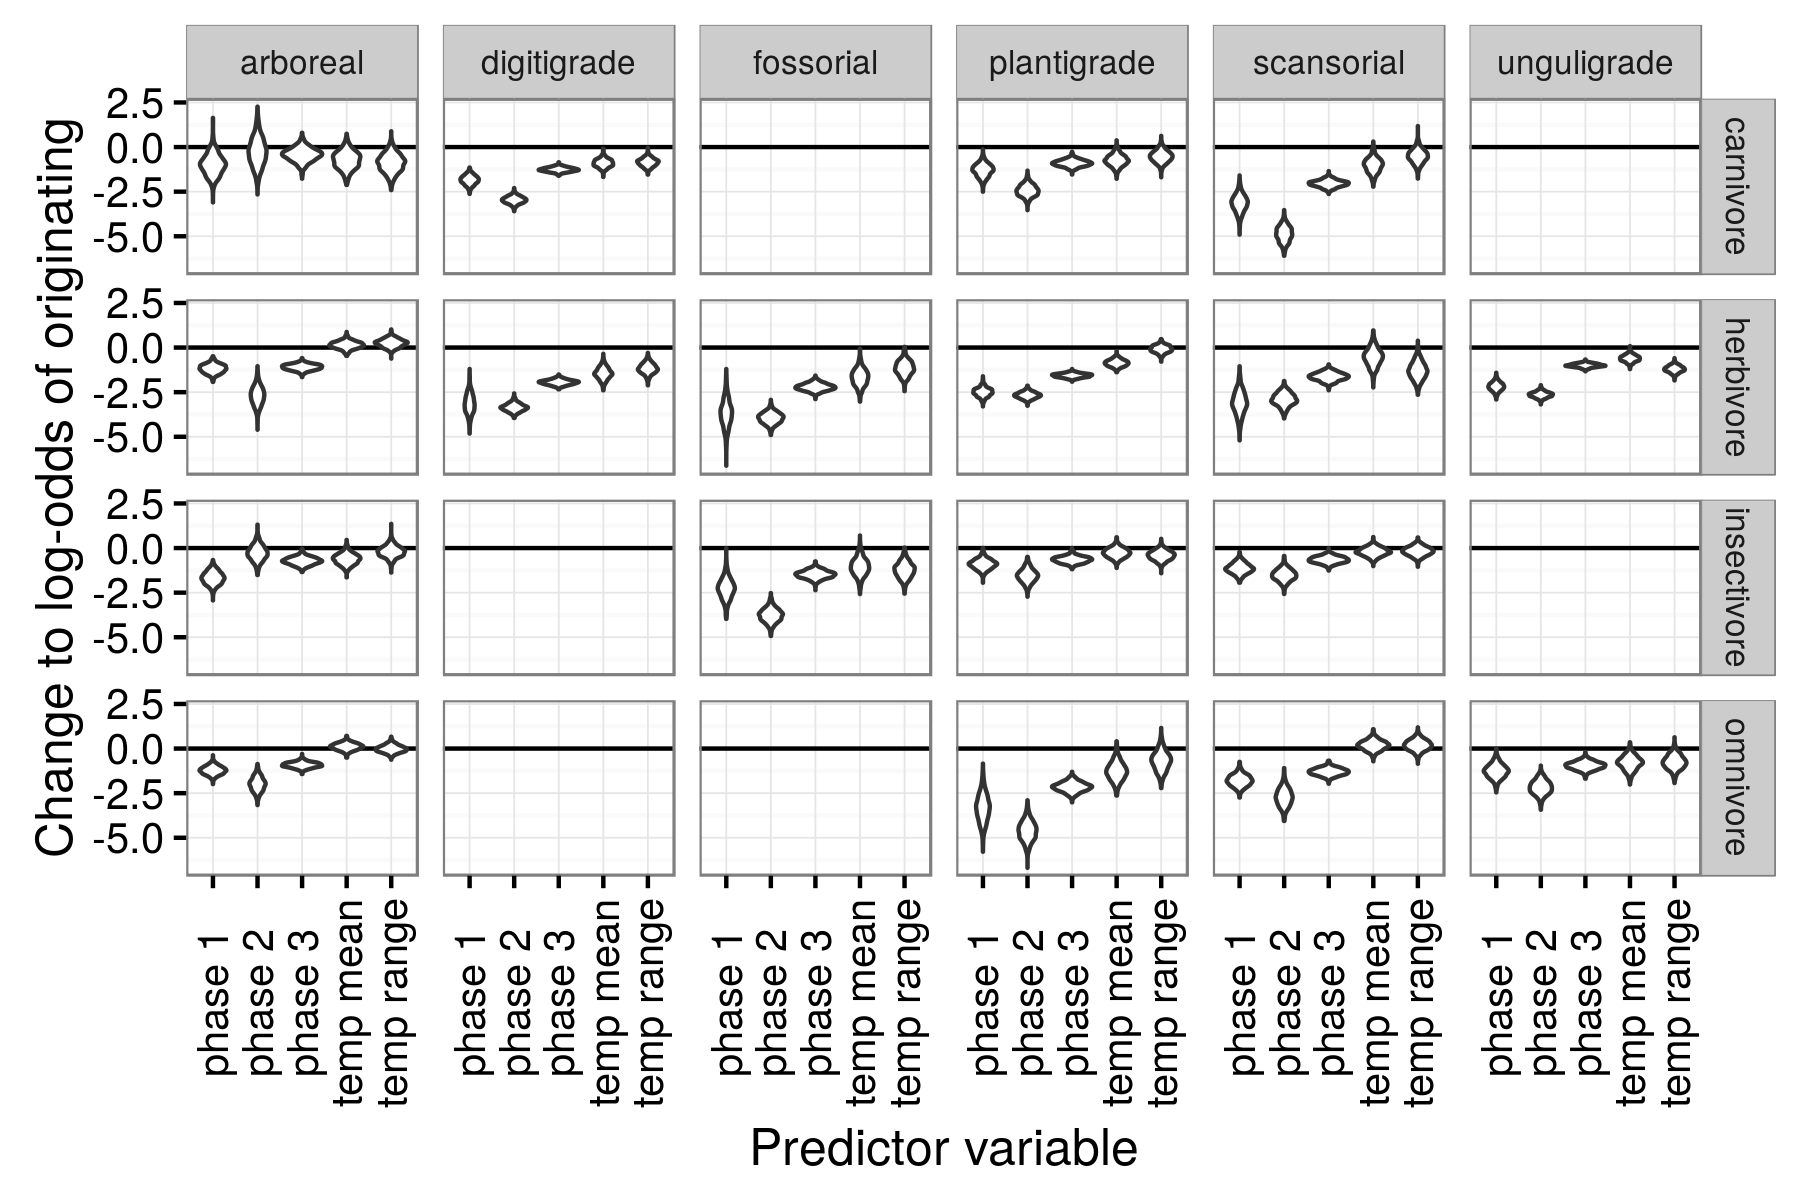
\includegraphics[width=\textwidth,height=0.4\textheight,keepaspectratio=true]{figure/group_on_origin_bd}
  \caption[Effects of group-level covariates on log-odds of ecotype origination as estimated from the birth-death model]{Estimated effects of the group-level covariates describing environmental context on log-odds of species origination. These estimates are from the birth-death model. What is plotted is a violin of the distribution of 1000 samples from the approximate posterior. The effect of plant phase graphed here is calculated as Phase 1\( = \gamma_{phase\ 1}\), Phase 2\( = \gamma_{phase\ 1} + \gamma_{phase\ 2}\), and so on.} 
  \label{fig:group_origin_bd}
\end{figure}

\begin{figure}[ht]
  \centering
  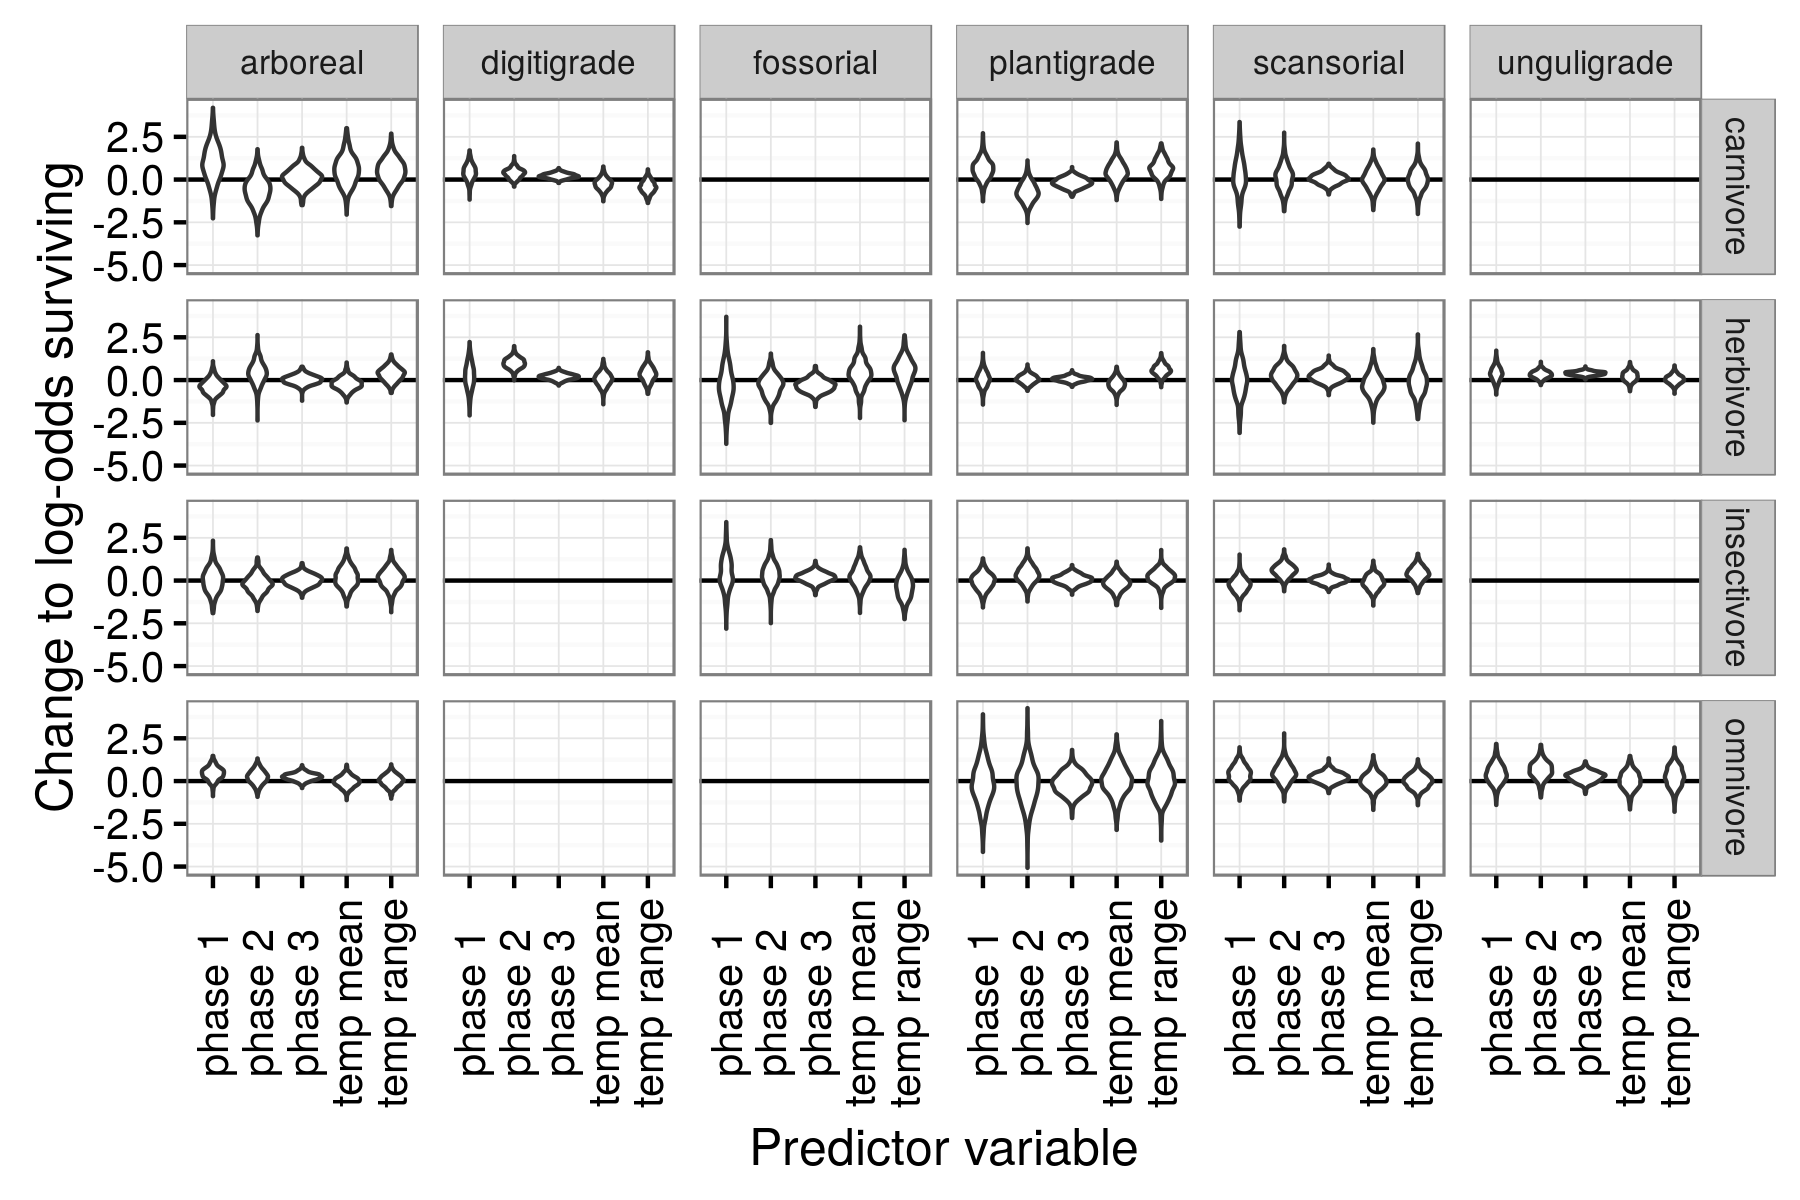
\includegraphics[width=\textwidth,height=0.4\textheight,keepaspectratio=true]{figure/group_on_survival_bd}
  \caption[Effects of group-level covariates on log-odds of ecotype survival as estimated from the birth-death model]{Estimated effects of the group-level covariates describing environmental context on log-odds of species survival. These estimates are from the birth-death model. What is plotted is a violin of the distribution of 1000 samples from the approximate posterior. The effect of plant phase graphed here is calculated as Phase 1\( = \gamma_{phase\ 1}\), Phase 2\( = \gamma_{phase\ 1} + \gamma_{phase\ 2}\), and so on.} 
  \label{fig:group_surv_bd}
\end{figure}



An association between plant phase and differences in the log-odds of occurrence (Fig. \ref{fig:group_pure_presence}), origination (Fig. \ref{fig:group_origin_bd}), or extinction (Fig. \ref{fig:group_surv_bd}) is interpreted to mean that the set of possible mammal-plant interactions was relatively more favorable (positive association) or less so (negative association) to those ecotypes. In the case of species origination, for example, more favorable conditions for an ecotype may indicate an increasing number of possible and available mammal-plant interactions (e.g. ecological opportunity; \citealp{Yoder2010,Losos2010,Losos2010a}); while adverse conditions may translate to a decreasing set of interactions or loss of appropriate environmental context. Remember that favorable versus adverse condition of a plant phase is definitionally relative to the other two plant phases. 

One of the limitations to this interpretation is the almost determistic increase in probability of occurrence and origination for most ecotypes (Fig. \ref{fig:eco_occur}, \ref{fig:eco_origin}). This ``pull of the Recent'' means that interpreting the biological meaning of differences between the final plant phase and the two previous phases is difficult as the guanteed occurrence of the later taxa increases the average probability for that phase, which in turn affects the other time bins in that phase.

Plant phases are associated with large differences in log-odds for occurrence and origination probabilities (Tables \ref{tab:occur_plant}, \ref{tab:origin_plant}), though there is little evidence of plant phase being an important distinguishing factor in species survival, as only a few ecotypes demonstrate strong affinities with some plant phases (Table \ref{tab:surv_plant}). 

The effects of plant phase on occurrence and origination probabilities are broadly congruent with each other (Fig. \ref{fig:group_pure_presence}, \ref{fig:group_origin_bd}). The almost universal pattern of the effect of plant phase on ecotype origination is that the during first and last plant phases ecotypes have a greater log-odds of occurrence or origination than the second plant phase (Fig. \ref{fig:eco_occur}, \ref{fig:eco_origin}). The three ecotypes that do not follow this pattern are fossorial herbivores, scansorial herbivores, and arboreal insectivores.


\begin{table}[ht]
  \centering
  \caption[Posterior probablity estimates of differences in occurrence by plant phase]{Posterior probability of the differences in the log-odds of an ecotype occurring based on plant phase. These probabilities are calculated as P(Phase 1 \(>\) 2) = \( (\sum \gamma_{phase 1} > \gamma_{phase 1} + \gamma_{phase 2}) / 100\) and similarly for the other comparisons. These estimates are from the pure-presence model.}
  \label{tab:occur_plant}
  \begin{tabular}{ l r r r }
    \hline
    & P(Phase 1 $>$ Phase 2) & P(Phase 2 $>$ Phase 3) & P(Phase 1 $>$ Phase 3) \\ 
    \hline
    arboreal carnivore & 0.323 & 0.874 & 0.926 \\ 
    digitigrade carnivore & 1.000 & 0.000 & 1.000 \\ 
    plantigrade carnivore & 1.000 & 0.040 & 1.000 \\ 
    scansorial carnivore & 1.000 & 0.015 & 1.000 \\ 
    arboreal herbivore & 1.000 & 0.515 & 1.000 \\ 
    digitigrade herbivore & 1.000 & 0.995 & 1.000 \\ 
    fossorial herbivore & 1.000 & 0.923 & 1.000 \\ 
    plantigrade herbivore & 1.000 & 0.995 & 1.000 \\ 
    scansorial herbivore & 1.000 & 0.717 & 1.000 \\ 
    unguligrade herbivore & 1.000 & 0.000 & 1.000 \\ 
    arboreal insectivore & 0.024 & 0.999 & 0.997 \\ 
    fossorial insectivore & 1.000 & 0.000 & 1.000 \\ 
    plantigrade insectivore & 0.923 & 0.558 & 0.985 \\ 
    scansorial insectivore & 0.982 & 0.483 & 0.992 \\ 
    arboreal omnivore & 0.959 & 0.837 & 1.000 \\ 
    plantigrade omnivore & 1.000 & 0.247 & 1.000 \\ 
    scansorial omnivore & 0.983 & 0.861 & 1.000 \\ 
    unguligrade omnivore & 1.000 & 0.189 & 0.998 \\ 
    \hline
  \end{tabular}
\end{table}

\begin{table}[ht]
  \centering
  \caption[Posterior probablity estimates of differences in origination by plant phase]{Posterior probability of the differences in the log-odds of an ecotype originating based on plant phase. These probabilities are calculated as P(Phase 1 \(>\) 2) = \( (\sum \gamma_{phase 1} > \gamma_{phase 1} + \gamma_{phase 2}) / 100\) and similarly for the other comparisons. These estimates are from the birth-death model.}
  \label{tab:origin_plant}
  \begin{tabular}{ l r r r }
    \hline
    & P(Phase 1 $>$ Phase 2) & P(Phase 2 $>$ Phase 3) & P(Phase 1 $>$ Phase 3) \\ 
    \hline
    arboreal carnivore & 0.405 & 0.777 & 0.905 \\ 
    digitigrade carnivore & 1.000 & 0.043 & 1.000 \\ 
    plantigrade carnivore & 1.000 & 0.053 & 1.000 \\ 
    scansorial carnivore & 1.000 & 0.035 & 1.000 \\ 
    arboreal herbivore & 1.000 & 0.163 & 1.000 \\ 
    digitigrade herbivore & 1.000 & 0.998 & 1.000 \\ 
    fossorial herbivore & 1.000 & 0.896 & 1.000 \\ 
    plantigrade herbivore & 1.000 & 0.996 & 1.000 \\ 
    scansorial herbivore & 1.000 & 0.884 & 1.000 \\ 
    unguligrade herbivore & 1.000 & 0.003 & 1.000 \\ 
    arboreal insectivore & 0.088 & 0.994 & 1.000 \\ 
    fossorial insectivore & 1.000 & 0.020 & 1.000 \\ 
    plantigrade insectivore & 0.995 & 0.419 & 1.000 \\ 
    scansorial insectivore & 0.999 & 0.360 & 1.000 \\ 
    arboreal omnivore & 0.999 & 0.317 & 1.000 \\ 
    plantigrade omnivore & 1.000 & 0.308 & 1.000 \\ 
    scansorial omnivore & 0.999 & 0.418 & 1.000 \\ 
    unguligrade omnivore & 1.000 & 0.219 & 1.000 \\ 
    \hline
  \end{tabular}
\end{table}


\begin{table}[ht]
  \centering
  \caption[Posterior probablity estimates of differences in survival by plant phase]{Posterior probability of the differences in the log-odds of an ecotype surviving based on plant phase. These probabilities are calculated as P(Phase 1 \(>\) 2) = \( (\sum \gamma_{phase 1} > \gamma_{phase 1} + \gamma_{phase 2}) / 100\) and similarly for the other comparisons. These estimates are from the birth-death model.}
  \label{tab:surv_plant}
  \begin{tabular}{ l r r r }
    \hline
    & P(Phase 1 $>$ Phase 2) & P(Phase 2 $>$ Phase 3) & P(Phase 1 $>$ Phase 3) \\ 
    \hline
    arboreal carnivore & 0.849 & 0.127 & 0.313 \\ 
    digitigrade carnivore & 0.292 & 0.411 & 0.162 \\ 
    plantigrade carnivore & 0.926 & 0.243 & 0.790 \\ 
    scansorial carnivore & 0.409 & 0.544 & 0.453 \\ 
    arboreal herbivore & 0.250 & 0.733 & 0.480 \\ 
    digitigrade herbivore & 0.000 & 0.990 & 0.246 \\ 
    fossorial herbivore & 0.547 & 0.680 & 0.812 \\ 
    plantigrade herbivore & 0.404 & 0.555 & 0.480 \\ 
    scansorial herbivore & 0.534 & 0.277 & 0.204 \\ 
    unguligrade herbivore & 0.600 & 0.046 & 0.003 \\ 
    arboreal insectivore & 0.673 & 0.379 & 0.539 \\ 
    fossorial insectivore & 0.464 & 0.442 & 0.308 \\ 
    plantigrade insectivore & 0.216 & 0.714 & 0.446 \\ 
    scansorial insectivore & 0.019 & 0.923 & 0.382 \\ 
    arboreal omnivore & 0.394 & 0.440 & 0.242 \\ 
    plantigrade omnivore & 0.582 & 0.542 & 0.677 \\ 
    scansorial omnivore & 0.292 & 0.590 & 0.289 \\ 
    unguligrade omnivore & 0.212 & 0.555 & 0.183 \\ 
    \hline
  \end{tabular}
\end{table}


Both aspects of global temperature analyzed here are estimated to have strong effects on species occurrence and origination for most mammal ecotypes (Tables \ref{tab:occur_temp}, \ref{tab:origin_temp}). Similarity, the probability that temperature has a large effect on species extinction is very low for all ecotypes (Table \ref{tab:surv_temp}). The effects of the temperature covariates on ecotype occurrence and origination are estimated to be negative, which which means that as temperature decreases, occurrence or origination are expected to increase. In the case of survival, the only strong ecotype association for either of the temperature covariates is a positive relationship between temperature range and occurrence probabilities of with plantigrade herbivores (Tab. \ref{tab:surv_temp}).

\begin{table}[ht]
  \centering
  \caption[Posterior probablity of effects of temperature on occurrence]{Posterior probabilities that the effects of the two temperature covariates on the log-odds of an ecotype occurring are greater than 0. What is estimated is the probability that these estimates are greater than 0; high or low probabilities indicate the ``strength'' of the covariate in that direction (positive and negative, respectively). These estimates are from the pure-presence model.}
  \label{tab:occur_temp}
  \begin{tabular}{ l r r }
    \hline
    & \(P(\gamma_{temp\ mean} > 0)\) & \(P(\gamma_{temp\ range} > 0)\) \\ 
    \hline
    arboreal carnivore & 0.067 & 0.043 \\ 
    digitigrade carnivore & 0.000 & 0.000 \\ 
    plantigrade carnivore & 0.012 & 0.054 \\ 
    scansorial carnivore & 0.007 & 0.086 \\ 
    arboreal herbivore & 0.762 & 0.852 \\ 
    digitigrade herbivore & 0.000 & 0.000 \\ 
    fossorial herbivore & 0.000 & 0.002 \\ 
    plantigrade herbivore & 0.000 & 0.364 \\ 
    scansorial herbivore & 0.141 & 0.004 \\ 
    unguligrade herbivore & 0.001 & 0.000 \\ 
    arboreal insectivore & 0.031 & 0.251 \\ 
    fossorial insectivore & 0.014 & 0.002 \\ 
    plantigrade insectivore & 0.164 & 0.058 \\ 
    scansorial insectivore & 0.197 & 0.250 \\ 
    arboreal omnivore & 0.711 & 0.449 \\ 
    plantigrade omnivore & 0.009 & 0.103 \\ 
    scansorial omnivore & 0.754 & 0.732 \\ 
    unguligrade omnivore & 0.015 & 0.022 \\ 
    \hline
  \end{tabular}
\end{table}



\begin{table}[ht]
  \centering
  \caption[Posterior probablity of effects of temperature on origination]{Posterior probability that the effects of the two temperature covariates on the log-odds of an ecotype origination are greater than 0. What is estimated is the probability that these estimates are greater than 0; high or low probabilities indicate the ``strength'' of the covariate in that direction (positive and negative, respectively). These estimates are from the birth-death model.}
  \label{tab:origin_temp}
  \begin{tabular}{ l r r }
    \hline
    & \(P(\gamma_{temp\ mean} > 0)\) & \(P(\gamma_{temp\ range} > 0)\) \\ 
    \hline
    arboreal carnivore & 0.072 & 0.031 \\ 
    digitigrade carnivore & 0.000 & 0.001 \\ 
    plantigrade carnivore & 0.010 & 0.094 \\ 
    scansorial carnivore & 0.006 & 0.104 \\ 
    arboreal herbivore & 0.785 & 0.881 \\ 
    digitigrade herbivore & 0.000 & 0.000 \\ 
    fossorial herbivore & 0.001 & 0.007 \\ 
    plantigrade herbivore & 0.000 & 0.626 \\ 
    scansorial herbivore & 0.097 & 0.002 \\ 
    unguligrade herbivore & 0.010 & 0.000 \\ 
    arboreal insectivore & 0.018 & 0.319 \\ 
    fossorial insectivore & 0.008 & 0.003 \\ 
    plantigrade insectivore & 0.223 & 0.084 \\ 
    scansorial insectivore & 0.139 & 0.202 \\ 
    arboreal omnivore & 0.646 & 0.628 \\ 
    plantigrade omnivore & 0.013 & 0.120 \\ 
    scansorial omnivore & 0.688 & 0.735 \\ 
    unguligrade omnivore & 0.016 & 0.027 \\ 
    \hline
  \end{tabular}
\end{table}

\begin{table}[ht]
  \centering
  \caption[Posterior probablity of effects of temperature on survival]{Posterior probability that the effects of the two temperature covariates on the log-odds of an ecotype survival are greater than 0. What is estimated is the probability that these estimates are greater than 0; high or low probabilities indicate the ``strength'' of the covariate in that direction (positive and negative, respectively). These estimates are from the birth-death model.}
  \label{tab:surv_temp}
  \begin{tabular}{ l r r }
    \hline
    & \(P(\gamma_{temp\ mean} > 0)\) & \(P(\gamma_{temp\ range} > 0)\) \\ 
    \hline
    arboreal carnivore & 0.751 & 0.752 \\ 
    digitigrade carnivore & 0.161 & 0.110 \\ 
    plantigrade carnivore & 0.851 & 0.878 \\ 
    scansorial carnivore & 0.598 & 0.510 \\ 
    arboreal herbivore & 0.281 & 0.819 \\ 
    digitigrade herbivore & 0.546 & 0.721 \\ 
    fossorial herbivore & 0.751 & 0.766 \\ 
    plantigrade herbivore & 0.316 & 0.960 \\ 
    scansorial herbivore & 0.342 & 0.429 \\ 
    unguligrade herbivore & 0.750 & 0.418 \\ 
    arboreal insectivore & 0.572 & 0.579 \\ 
    fossorial insectivore & 0.648 & 0.279 \\ 
    plantigrade insectivore & 0.477 & 0.786 \\ 
    scansorial insectivore & 0.303 & 0.845 \\ 
    arboreal omnivore & 0.536 & 0.611 \\ 
    plantigrade omnivore & 0.499 & 0.507 \\ 
    scansorial omnivore & 0.544 & 0.488 \\ 
    unguligrade omnivore & 0.520 & 0.688 \\ 
    \hline
  \end{tabular}
\end{table}





The apparent similarities in origination rate of digitgrade carnivores, digitigrade herbivores, plantigrade herbivores, and unguligrade herbivores (Fig. \ref{fig:eco_origin} can be tested by inspecting the estimates of the two correlation matrices \(\Omega^{\phi}\) and \(\Omega^{\pi}\). The elements of these matrices are estimates of the correlation in origination and survival probabilities, respectively, between each of the 18 observed ecotypes. However, because ADVI-based inference assumes that the joint posterior is Gaussian, estimates of scale and correlation parameters are very approximate as these parameters tend to have decidedly non-Gaussian true posterior distributions \citep{Gelman2013d}. Because of this fundamental limitation, inference based on these correlation matrices are very approximate and subject to change.

Consistent with visual inspection of the ecotype origination probability time series, there are some strong positive correlations between a few ecotypes (Fig. \ref{fig:origin_corr}). Given the posterior distribution of correlation estimates, the probability of these correlation estimates being greater than 0 can be estimated. Again, because of the assumed Gaussian posterior, these probability estimates are at best approximate and are subject to change given full posterior inference. To visualize these results, I've plotted an association graph of the correlations between ecotypes that are estimated to have a greater than 95\% posterior probability of being greater than 0 (Fig. \ref{fig:origin_corr_graph}); in total there are 35 correlations that fit this criterion. The ecotypes correlated with the most number of other ecotyes, in order from most to least, are unguligrade herbivores, plantigrade herbivores, digitigrade carnivores, scansorial carnivore, fossorial herbivores, and plantigrade omnivores. These results support the conclusion that the origination probabilities of many ecotypes are correlated which I interpret to mean that changes to the species pool's environment context can lead to the simultaneous enrichment of multiple ecotypes instead of each ecotype respondingly independently. This result is most obvious for digitigrade carnivores, scansorial carnivores, digitigrade herbivores, fossorial herbivores, plantigrade herbivores, and unguligrade herbivores; these ecotypes are heavily cross-correlated with each other.

\begin{figure}[ht]
  \centering
  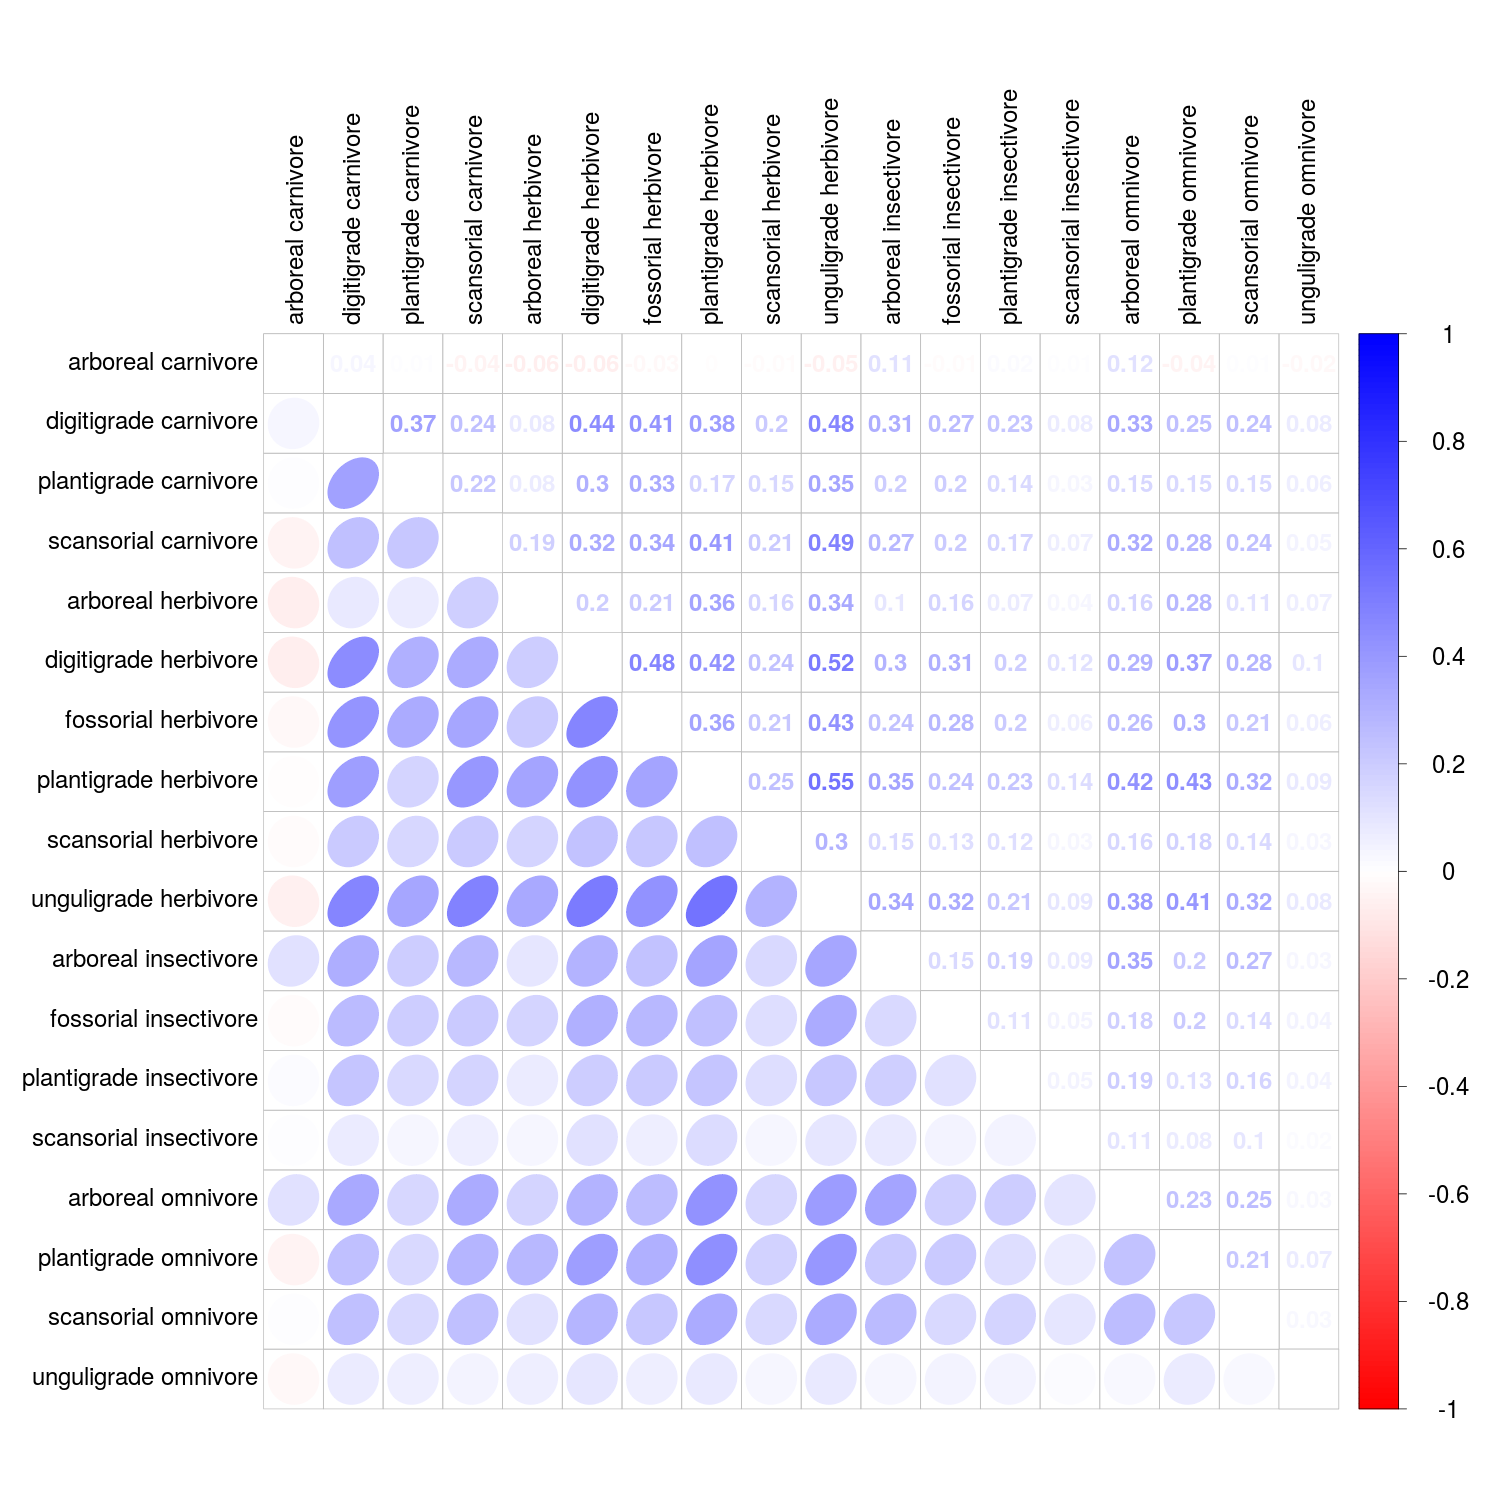
\includegraphics[width=\textwidth,height=\textheight,keepaspectratio=true]{figure/origination_correlation}
  \caption[Estimated correlations in origination probability between ecotypes]{Posterior mean estimates of the correlations in origination probability between the mammal ecotypes. The lower triangle of the matrix is populated with ellipses corresponding to the level of correlation between the two ecotypes, while the upper triangle of the matrix corresponds to the mean estimated correlation between ecotypes. Darker values correspond to a greater magnitude of correlation with blue values corresponding to a positive correlation and red values a negative correlation.}
  \label{fig:origin_corr}
\end{figure}

\begin{figure}[ht]
  \centering
  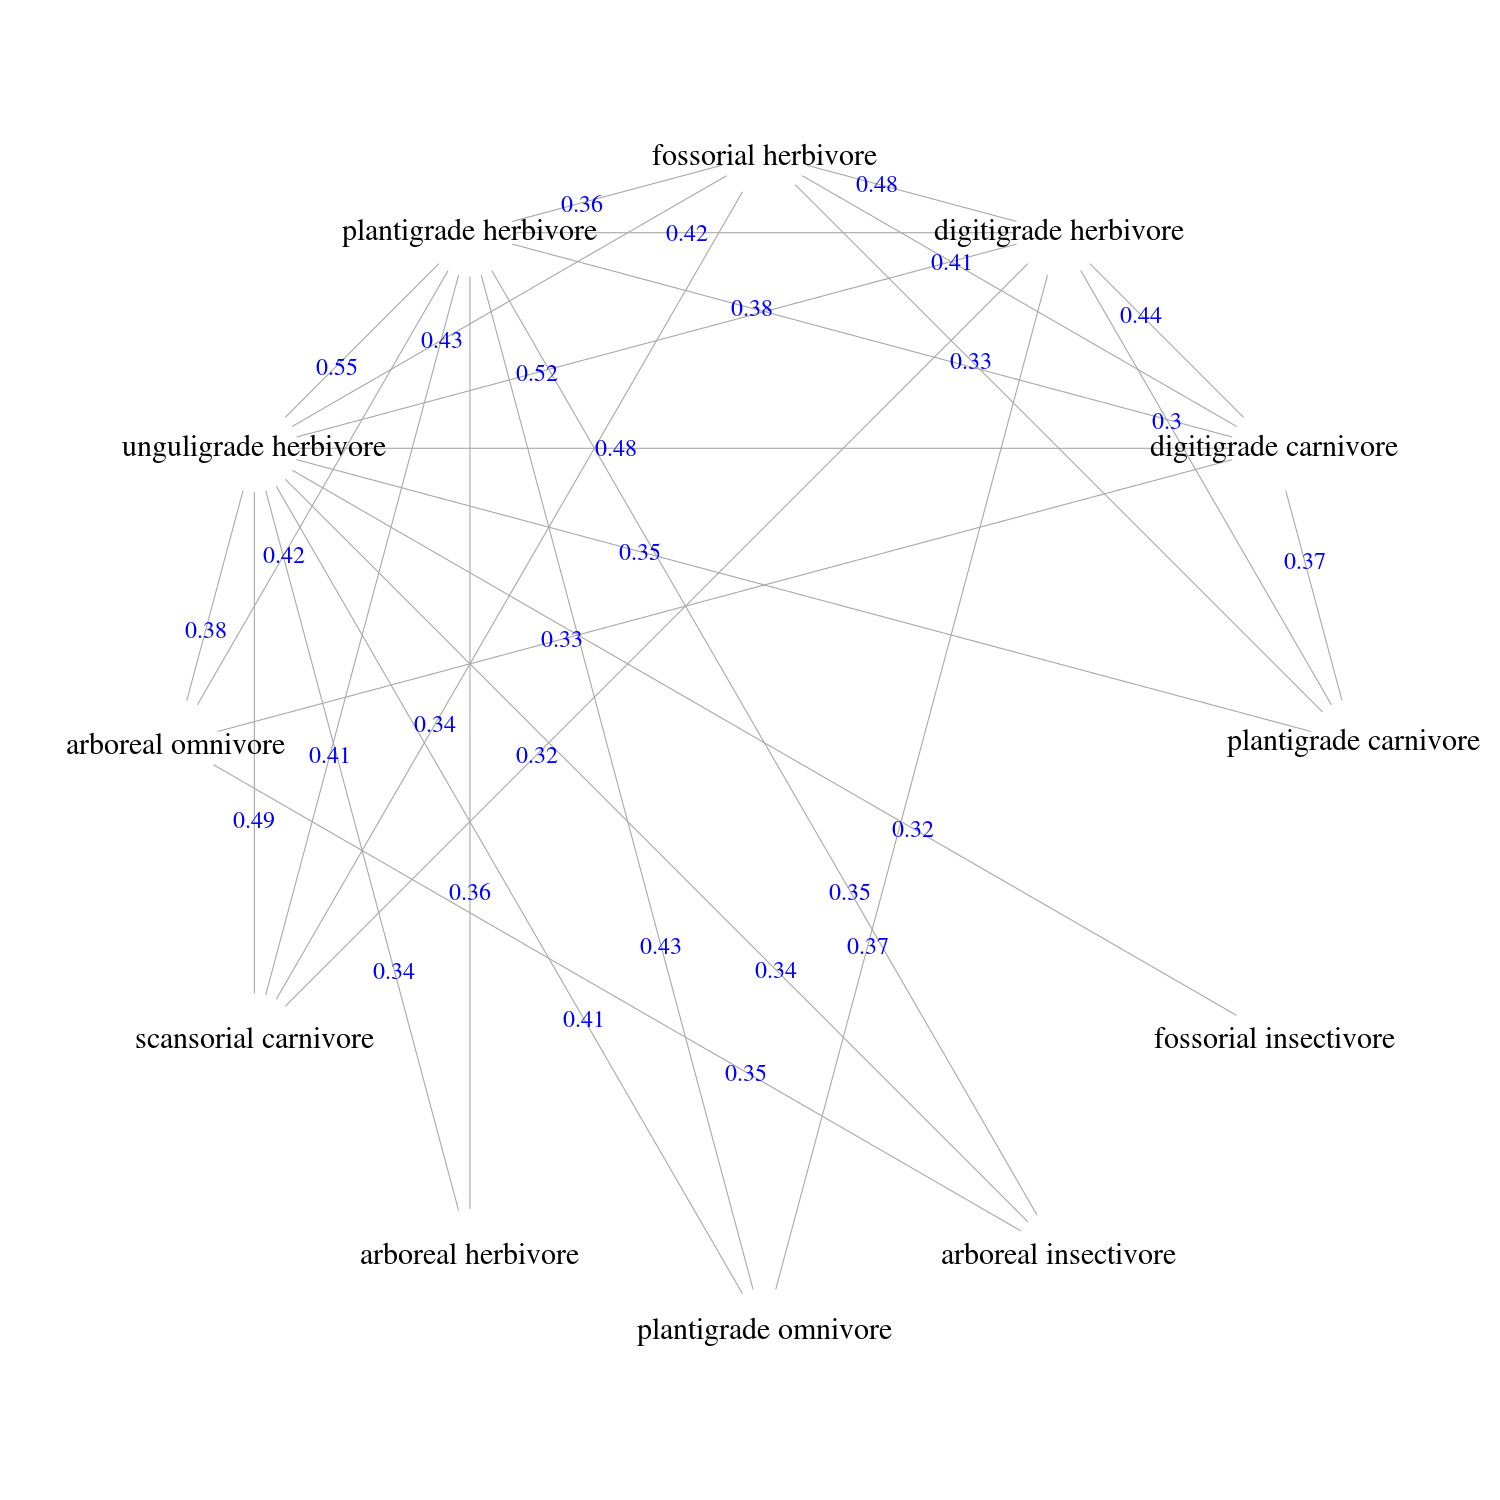
\includegraphics[width=\textwidth,height=\textheight,keepaspectratio=true]{figure/origin_sig_corr}
  \caption[Ecotypes with strong correlations in origination probability]{Ecotypes that have a strong correlation in origination probability. These ecotypes have a greater than 95\% posterior probability of being positively correlated. The number plotted at the midpoint of each edge corresponds to the mean estimated correlation between those two ecotypes.}
  \label{fig:origin_corr_graph}
\end{figure}


In contrast to the visually obvious correlations in ecotype origination probability, visual inspection of the ecotype-specific survival probabilities (Fig. \ref{fig:eco_survival}) does not indicate that many strong correlations between ecotype survival probabilities. This conclusion is supported by the estimated correlations in ecotype survival probability (Fig. \ref{fig:survival_corr}). There are very few large magnitude estimates of correlation between any of the ecotypes. This result is further supported by the fact that only a single correlation, survival probability of digitigrade carnivores and unguligrade herbivores, has a greater than 95\% posterior probability of being positive (Fig. \ref{fig:surv_corr_graph}). This single correlation, however, adds more nuance to the interpretations from the origination probability correlations. In addition to correlation in enrichment, these ecotypes are correlated in their depletions. This result supports the conclusion that the diversity history of digitigrade carnivores and unguligrade herbivores are strongly related to each other both in terms of origination and survival, which stands in contrast to those ecotypes which are only correlated for origination.


\begin{figure}[ht]
  \centering
  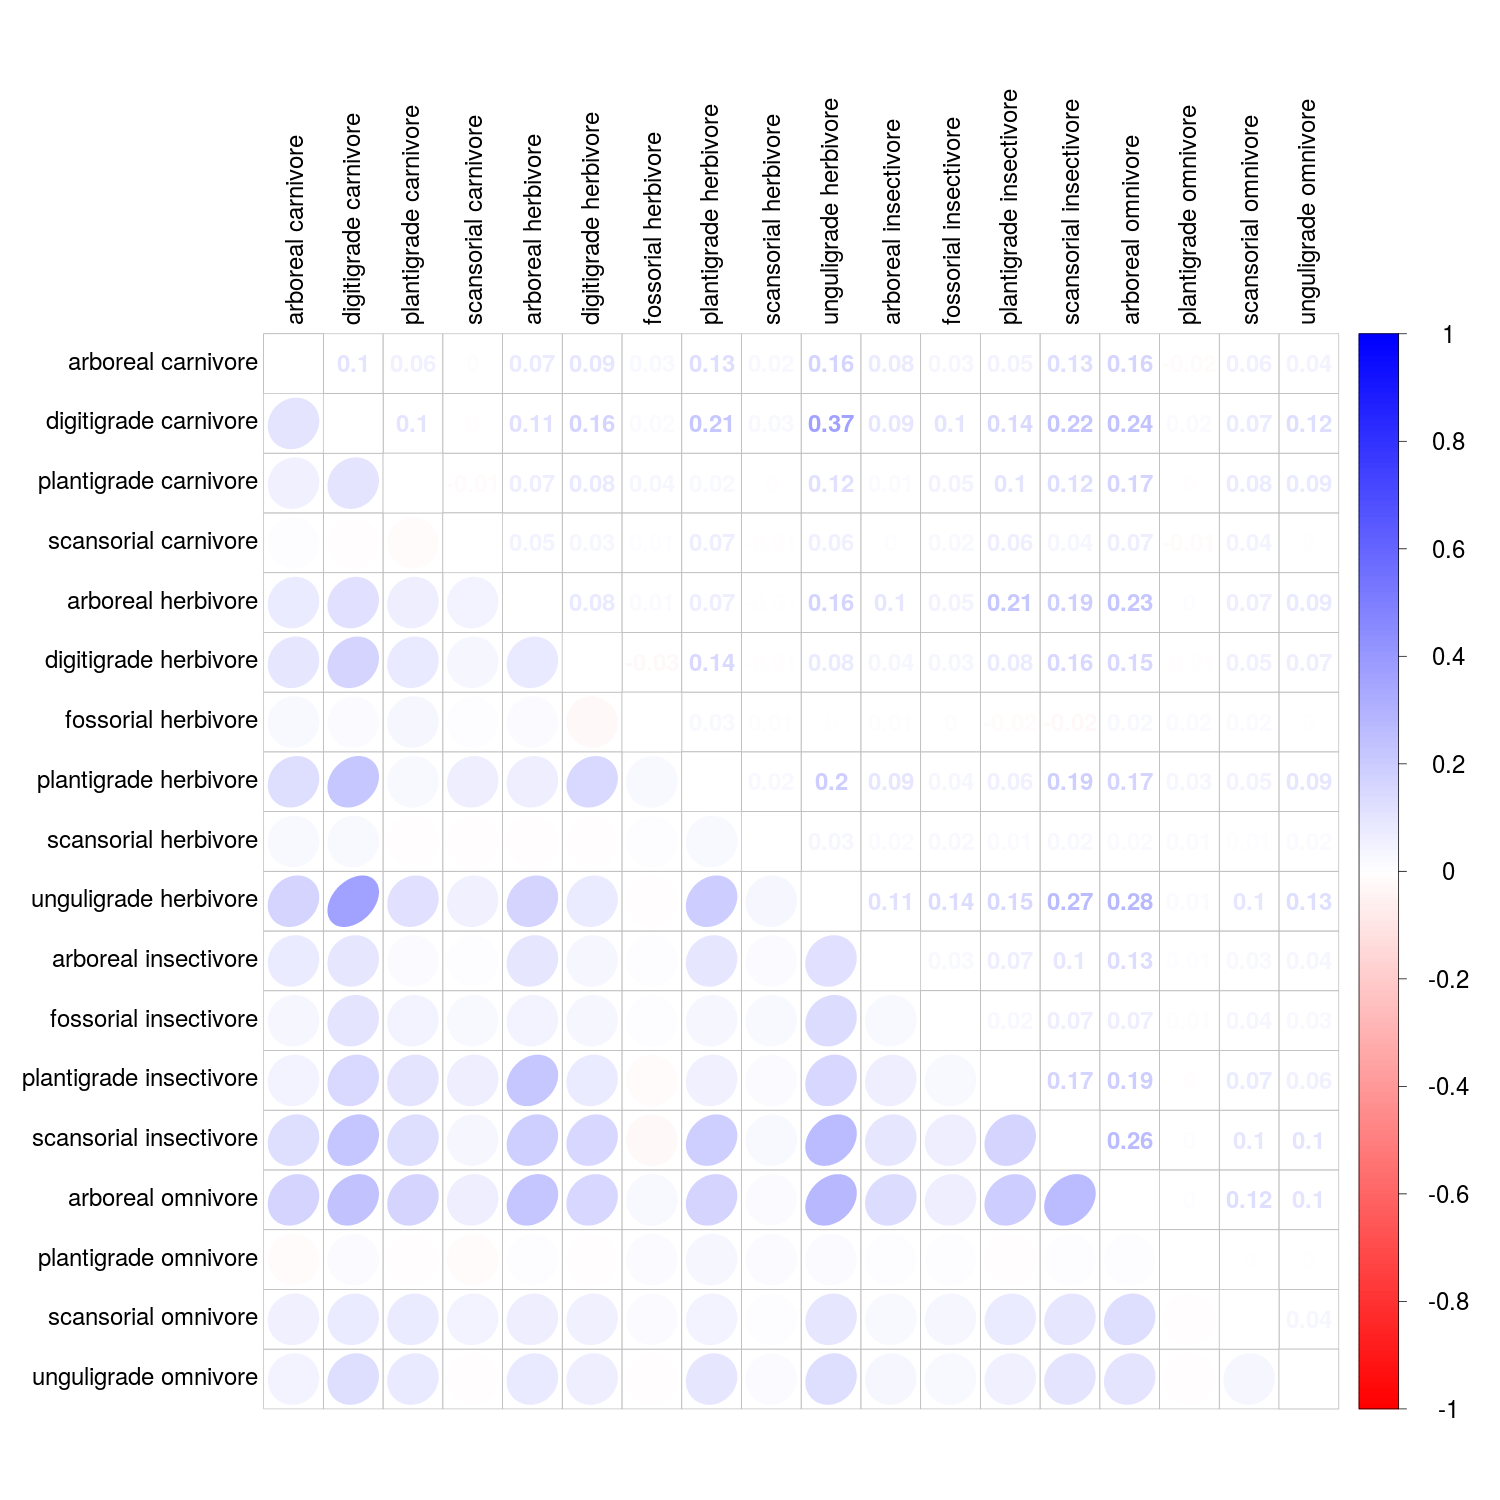
\includegraphics[width=\textwidth,height=\textheight,keepaspectratio=true]{figure/survival_correlation}
  \caption[Estimated correlations in survival probability between ecotypes]{Posterior mean estimates of the correlations in survival probability between the mammal ecotypes. The lower triangle of the matrix is populated with ellipses corresponding to the level of correlation between the two ecotypes, while the upper triangle of the matrix corresponds to the mean estimated correlation between ecotypes. Darker values correspond to a greater magnitude of correlation with blue values corresponding to a positive correlation and red values a negative correlation.}
  \label{fig:survival_corr}
\end{figure}

\begin{figure}[ht]
  \centering
  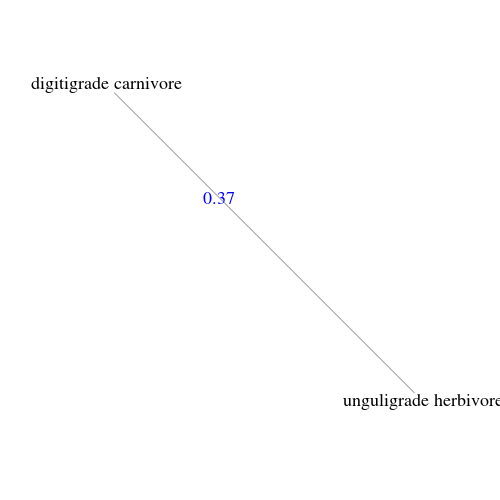
\includegraphics[width=\textwidth,height=0.4\textheight,keepaspectratio=true]{figure/surv_sig_corr}
  \caption[Ecotypes with strong correlations in survival probability]{Ecotypes that have a strong correlation in survival probability. These ecotypes have a greater than 95\% posterior probability of being positively correlated. The number plotted at the midpoint of each edge corresponds to the mean estimated correlation between those two ecotypes.}
  \label{fig:surv_corr_graph}
\end{figure}










\subsection*{Analysis of diversity}

All of the analyses of diversification and macroevolutionary rates has been done using only the birth-death model because of the model's better posterior predictive check performance (Fig. \ref{fig:ppc}).


The general pattern of the estimated North American total mammal diversity for the Cenozoic is ``stable'' in that diversity fluctuates around a constant mean standing diverisity, does not fluctuate wildly and rapidly over the Cenozoic, and demonstrates no sustained directional trends (Fig. \ref{fig:diversity_est}). In broad strokes, the first 15 or so million years of the Cenozoic are characterized by first an increase and then a decline in standing diversity at approximately 45-50 Mya (early-middle Eocene). Following this decline, standing diversity is broadly constant from 45 to 18 Mya (early Miocene). After this, there is a rapid spike in diversity followed by a slight decline in diversity up to the Recent. 

The pattern exhibited by the diversity history estimated in this study (Fig. \ref{fig:diversity_est}) has some major similarities with previous mammal diversity curves \citep{Alroy2009}: both curves begin with an increase in diversity most of the major increases in diversity are retained including the large diversity spike during the Miocene. Unlike subsampling based approaches to estimating diversity \citep{Alroy2010c}, I'm able to interpolate over unsampled/poorly sampled time periods because of how the hierarchical model can share information across the different units \cite{Gelman2013d}; for cases like unsampled temporal bins, this may lead to estimates with high uncertainty, but that is preferable to no estimate at all. Finally, the Bayesian framework here gives a distribution of possible estimates of diversity allowing for direct inspection of the uncertainty of our inferences, something that is preferable to both traditional and resampling based confidence interval estimates \citep{Gelman2013d}. Note that my time series of estimated diversity begins at a slightly different point than that of \citet{Alroy2009} and that the time intervals used by \citet{Alroy2009} are slightly shorter than those used here, so this may cause some of the minor differences between the curves. Also, please note that the diversity values are plotted at the ``ceiling'' of each temporal interval and not at the midpoint (Fig. \ref{fig:diversity_est}).

When viewed through the lens of diversification rate, some of the structure behind the estimated diversity history begins to take shape (Fig. \ref{fig:diversity_rate}). For most of the Cenozoic, the diversification rate hovers around zero, punctuated by both positive and negative spikes. The largest spike in diversification rate is at 16 Mya, which is early Oligocene (Fig. \ref{fig:diversity_rate}). Other notable increases in diversification rate occur 56, 46, 22, 18, and 6 Mya (Table \ref{tab:div_peak}), though the last of these may be due to edge effects surrounding the partial-identifiability of \(p_{t = T}\). Notable decreases in diversification rate occur at 54, 50, 48, 44, 40, 34, 30, 24, 20, 16, 12, and 8 Mya (Table \ref{tab:div_peak}), meaning that diversification rate has more major decreases than increases. While diversification rates significantly lower than average are more common than diversification rates greater than average, when diversification rate does increases it is with a greater magnitude than most decreases (Fig. \ref{fig:diversity_rate}). Given that diversification rate more closely resembles origination rate than extinction rate (Fig. \ref{fig:diversity_rate}, \ref{fig:origin_rate}, \ref{fig:extinct_rate}), these decreases in diversification rate may be indicative of ``depletions'' (failure to replace extinct taxa) rather than pulses of extinction. 

The estimates from this study of per capita origination and extinction rates for the entire species pool (Fig. \ref{fig:origin_rate}, \ref{fig:extinct_rate}) are very different from the origination and extinction rates estimated by \citet{Alroy2009}. The two most striking difference are the very different estimates of extinction rate between the two studies and the very different scales of the origination rate estimates. This may be due to the fundamentally different way these rates are calculated, and how the diversification process was modeled. The per capita rates estimated in this study follow straight from the definition of a per capita rate (e.g. number of originations between time \(t\) and \(t + 1\) divided by the diversity at time \(t\)) while the rates calculated in \citet{Alroy2009} are based on log ratios of standing diversity.

The comparison between per capita origination and extinction rate estimates reveals how diversification rate is formed (Fig. \ref{fig:origin_rate}, \ref{fig:extinct_rate}). As expected given previous inspection of the ecotype specific estimates of origination and survival probabilities from the birth-death model, diversification rate seems most driven by changes in origination rate as opposed to extinction rate. Extinction rate, on the other hand, demonstrates an almost saw-toothed pattern around a constant mean (Fig. \ref{fig:extinct_rate}). These results are broadly consistent with those from previous analyses of North American mammals diversity and diversification \citep{Alroy1996a,Alroy2000g,Alroy2009}.


\begin{figure}[ht]
  \begin{subfigure}[b]{0.45\textwidth}
    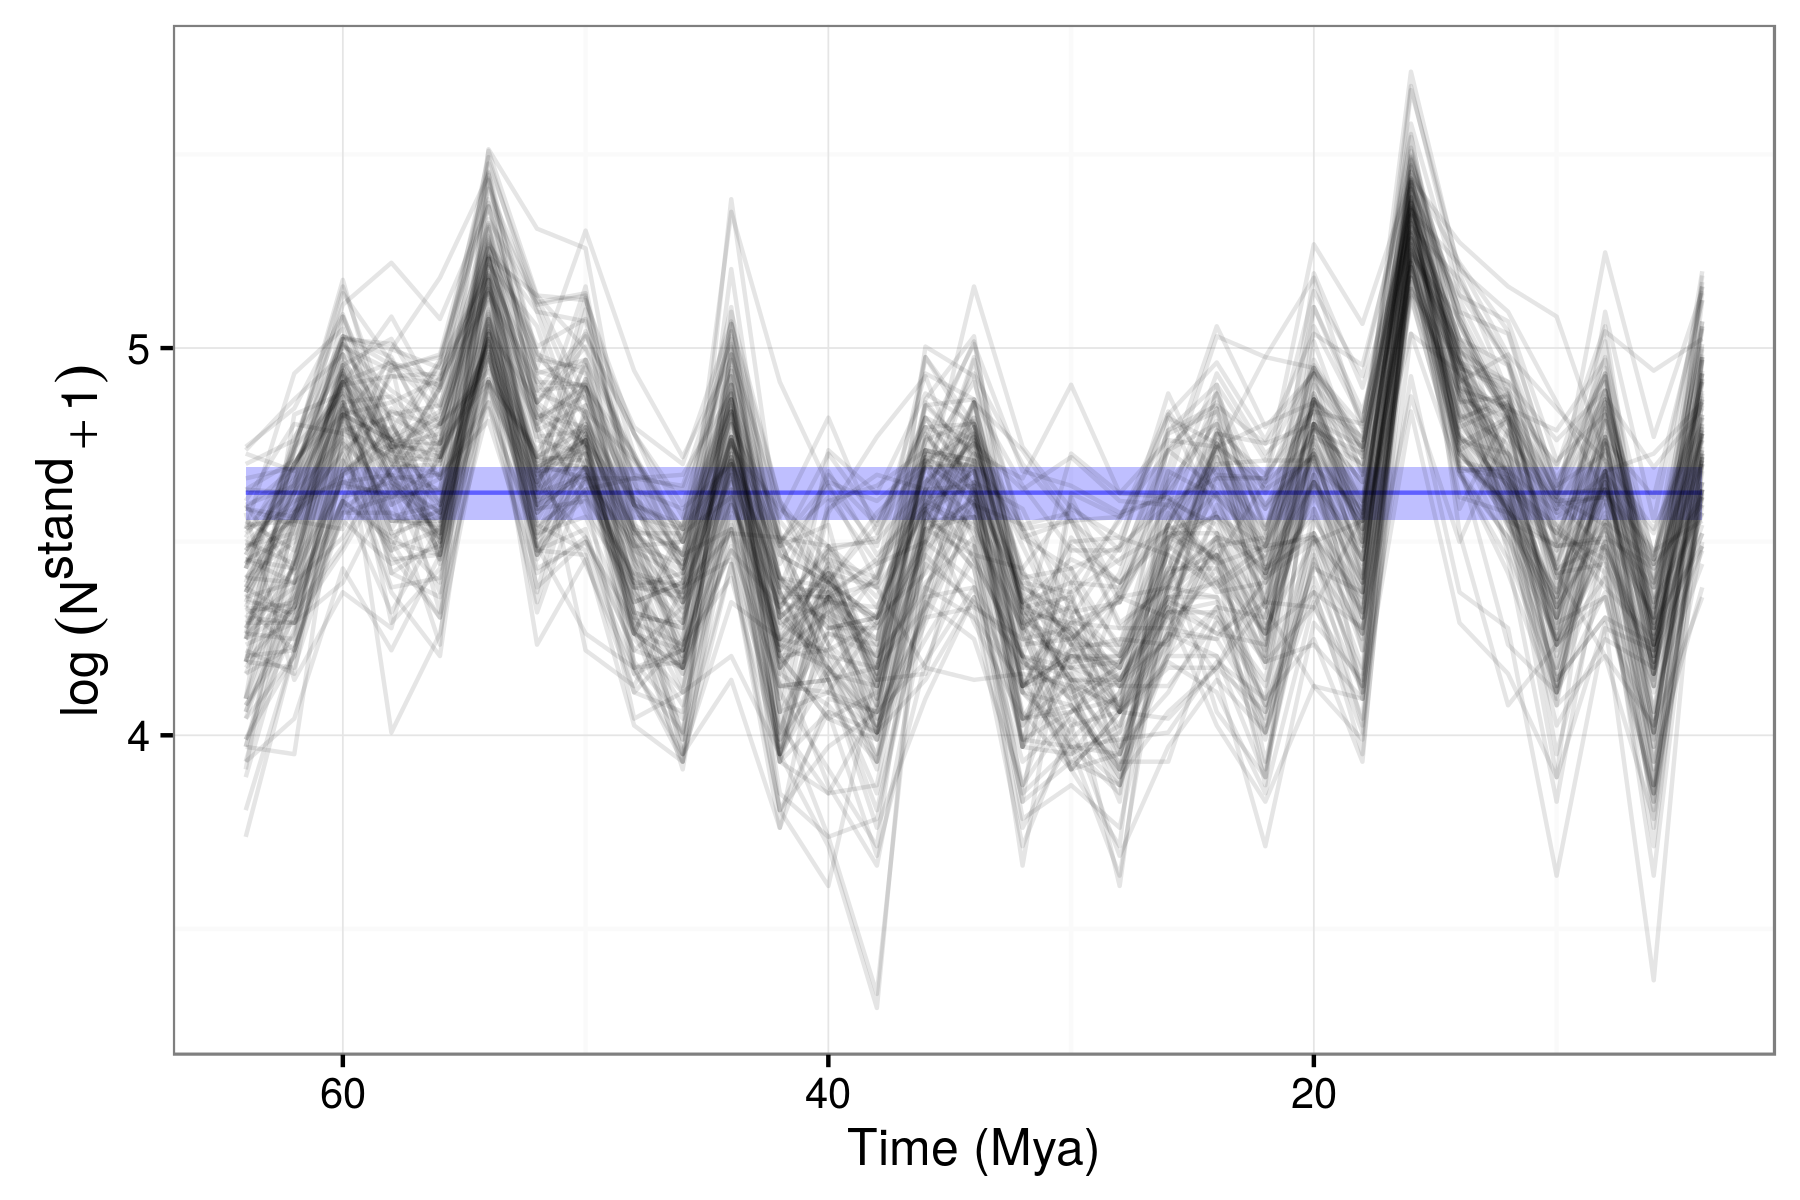
\includegraphics[width=\textwidth,height=0.4\textheight,keepaspectratio=true]{figure/log_diversity}
    \caption{Log diversity}
    \label{fig:diversity_est}
  \end{subfigure}
  \begin{subfigure}[b]{0.45\textwidth}
    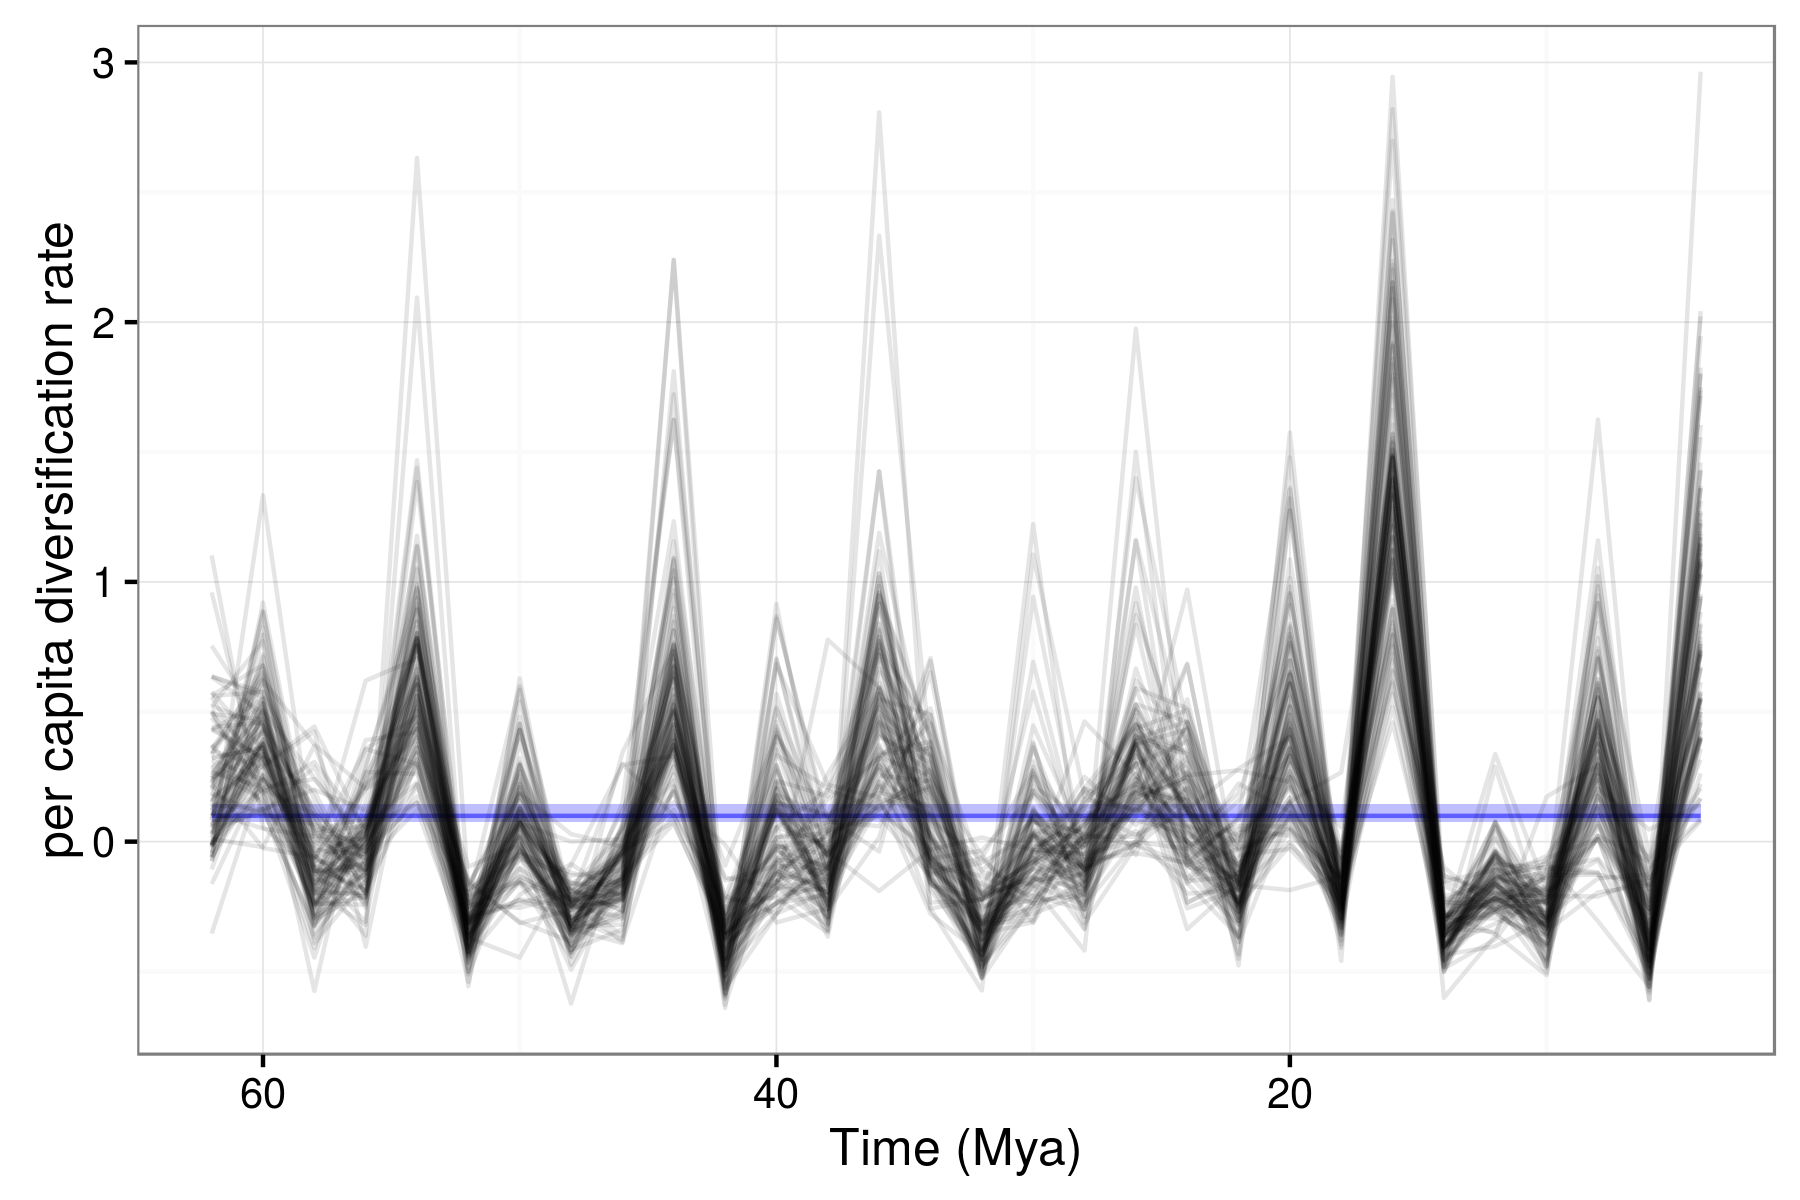
\includegraphics[width=\textwidth,height=0.4\textheight,keepaspectratio=true]{figure/div_rate}
    \caption{Diversification rate}
    \label{fig:diversity_rate}
  \end{subfigure}

  \begin{subfigure}[b]{0.45\textwidth}
    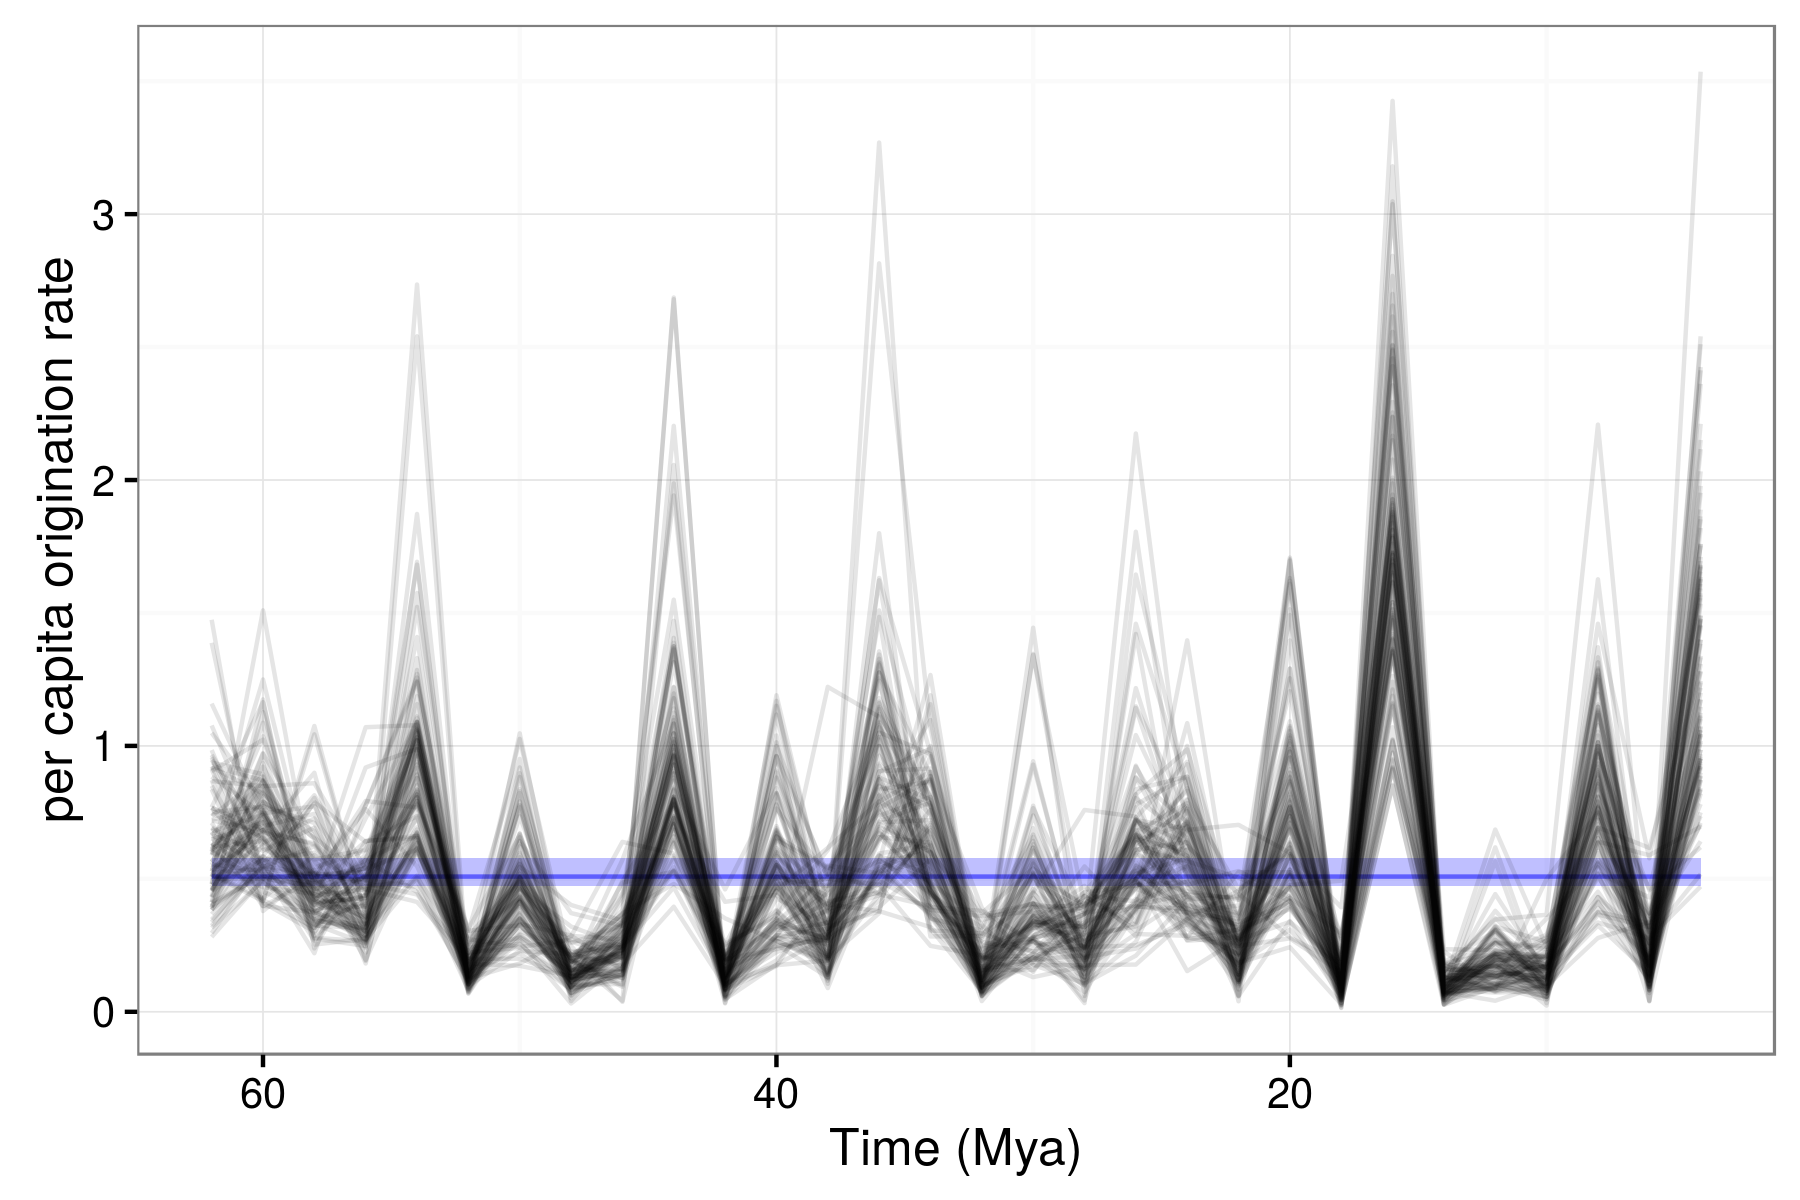
\includegraphics[width=\textwidth,height=0.4\textheight,keepaspectratio=true]{figure/orig_rate}
    \caption{Origination rate}
    \label{fig:origin_rate}
  \end{subfigure}
  \begin{subfigure}[b]{0.45\textwidth}
    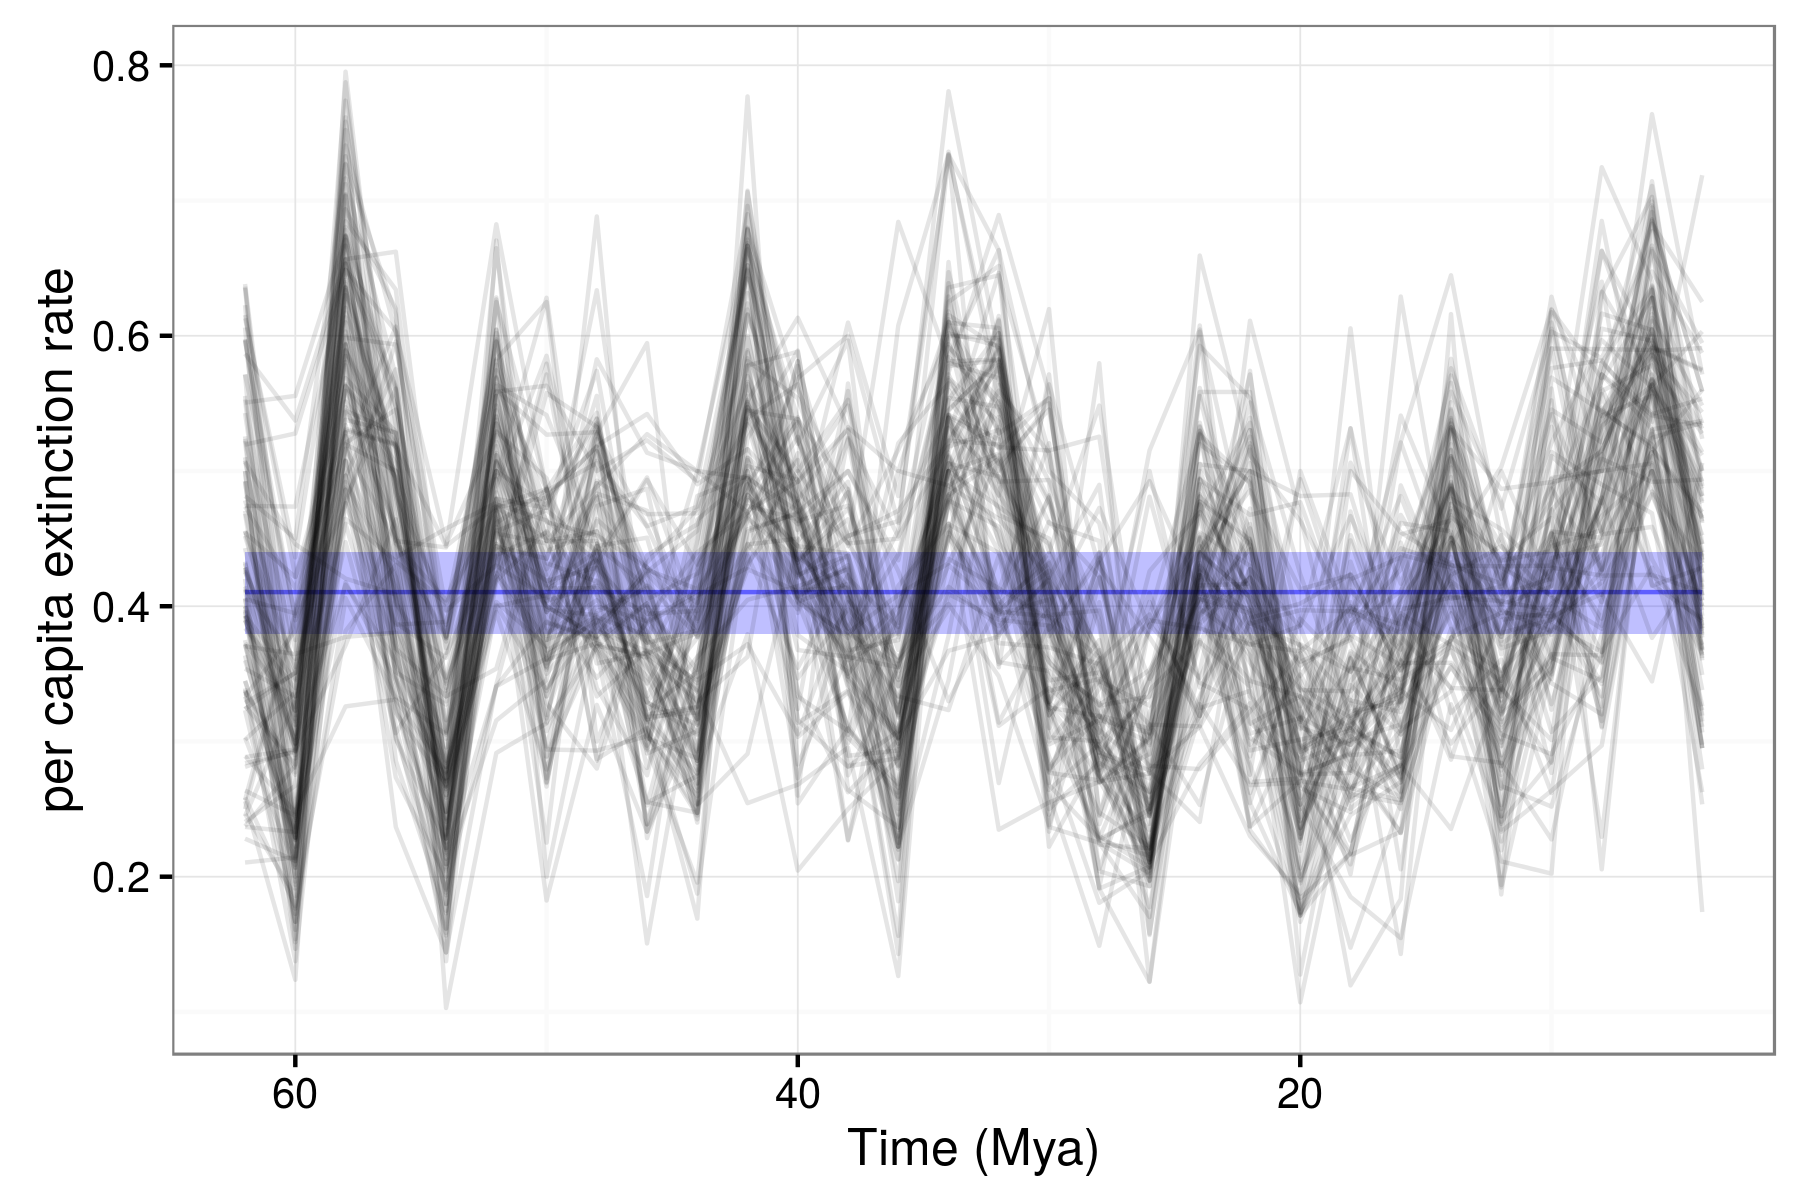
\includegraphics[width=\textwidth,height=0.4\textheight,keepaspectratio=true]{figure/death_rate}
    \caption{Extinction rate}
    \label{fig:extinct_rate}
  \end{subfigure}
  \caption[Estimated mammal log-diversity and macroevolutionary rates for the Cenozoic]{Posterior estimates of the time series of Cenozoic North American mammal diversity and it's characteristic macroevolutionary rates; all estimates are from the birth-death model and 100 posterior draws are plotted to indicate the uncertainty in these estimates. The blue horizontal strip corresponds to the 80\% credible interval of estimated mean standing diversity, diversification rate, origination rate, and extinction rate respectively; the median estimate is also indicated. What is also plotted is the  The dramatic differences between diversity estimates at the first and second time points and the penultimate and last time points in this series are caused by well known edge effects in discrete-time birth-death models caused by \(p_{\_, t = 1}\) and \(p_{\_, t = T}\) being partially unidentifiable \citep{Royle2008}; the hierarchical modeling strategy used here helps mitigate these effects but they are still present \citep{Gelman2013d,Royle2008}. Diversification rate is in units of species gained per species present per time unit (2 My), origination rate is in units of species originating per species present per time unit, and extinction rate is in units of species becoming extinct per species present per time unit.}
  \label{fig:macro_values}
\end{figure}

\begin{table}[ht]
  \centering
  \caption[Posterior probability estimates of a peak in diversity, diversification]{Posterior probabilities of diversity \(N^{stand}_{t}\) or diversification rate \(D^{rate}_{t}\) being greater than average standing diversity \(\overline{N^{stand}}\) or average diversification rate \(\overline{D^{rate}}\) for the whole Cenozoic. The ``Time'' column corresponds to the top of each of the temporal bins. Diversification rate can not be estimated for the last time point because it is unknown how many more species originated or went extinct following this temporal bin. The estimates are from the birth-death model.}
  \label{tab:div_peak}
  \begin{tabular}{ r r r }
    \hline
    Time (Mya) & \(P(N^{stand}_{t} > \overline{N^{stand}})\) & \(P(D^{rate}_{t} > \overline{D^{rate}})\) \\ 
    \hline
    64.00 & 0.07 & 0.63 \\ 
    62.00 & 0.28 & 0.94 \\ 
    60.00 & 0.86 & 0.13 \\ 
    58.00 & 0.68 & 0.18 \\ 
    56.00 & 0.62 & 0.99 \\ 
    54.00 & 1.00 & 0.00 \\ 
    52.00 & 0.68 & 0.41 \\ 
    50.00 & 0.80 & 0.00 \\ 
    48.00 & 0.12 & 0.04 \\ 
    46.00 & 0.01 & 0.98 \\ 
    44.00 & 0.64 & 0.00 \\ 
    42.00 & 0.02 & 0.47 \\ 
    40.00 & 0.03 & 0.08 \\ 
    38.00 & 0.00 & 0.89 \\ 
    36.00 & 0.40 & 0.46 \\ 
    34.00 & 0.52 & 0.00 \\ 
    32.00 & 0.02 & 0.27 \\ 
    30.00 & 0.06 & 0.09 \\ 
    28.00 & 0.02 & 0.88 \\ 
    26.00 & 0.22 & 0.39 \\ 
    24.00 & 0.38 & 0.03 \\ 
    22.00 & 0.09 & 0.96 \\ 
    20.00 & 0.81 & 0.00 \\ 
    18.00 & 0.29 & 1.00 \\ 
    16.00 & 1.00 & 0.00 \\ 
    14.00 & 0.95 & 0.02 \\ 
    12.00 & 0.80 & 0.01 \\ 
    10.00 & 0.13 & 0.83 \\ 
    8.00 & 0.67 & 0.00 \\ 
    6.00 & 0.02 & 1.00 \\ 
    4.00 & 0.91 &  \\ 
    \hline
  \end{tabular}
\end{table}


Diversity partitioned by ecotype reveals a lot of the complexity behind the pattern of mammal diversity for the Cenozoic (Fig. \ref{fig:ecotype_diversity}). 

\begin{figure}[ht]
  \centering
  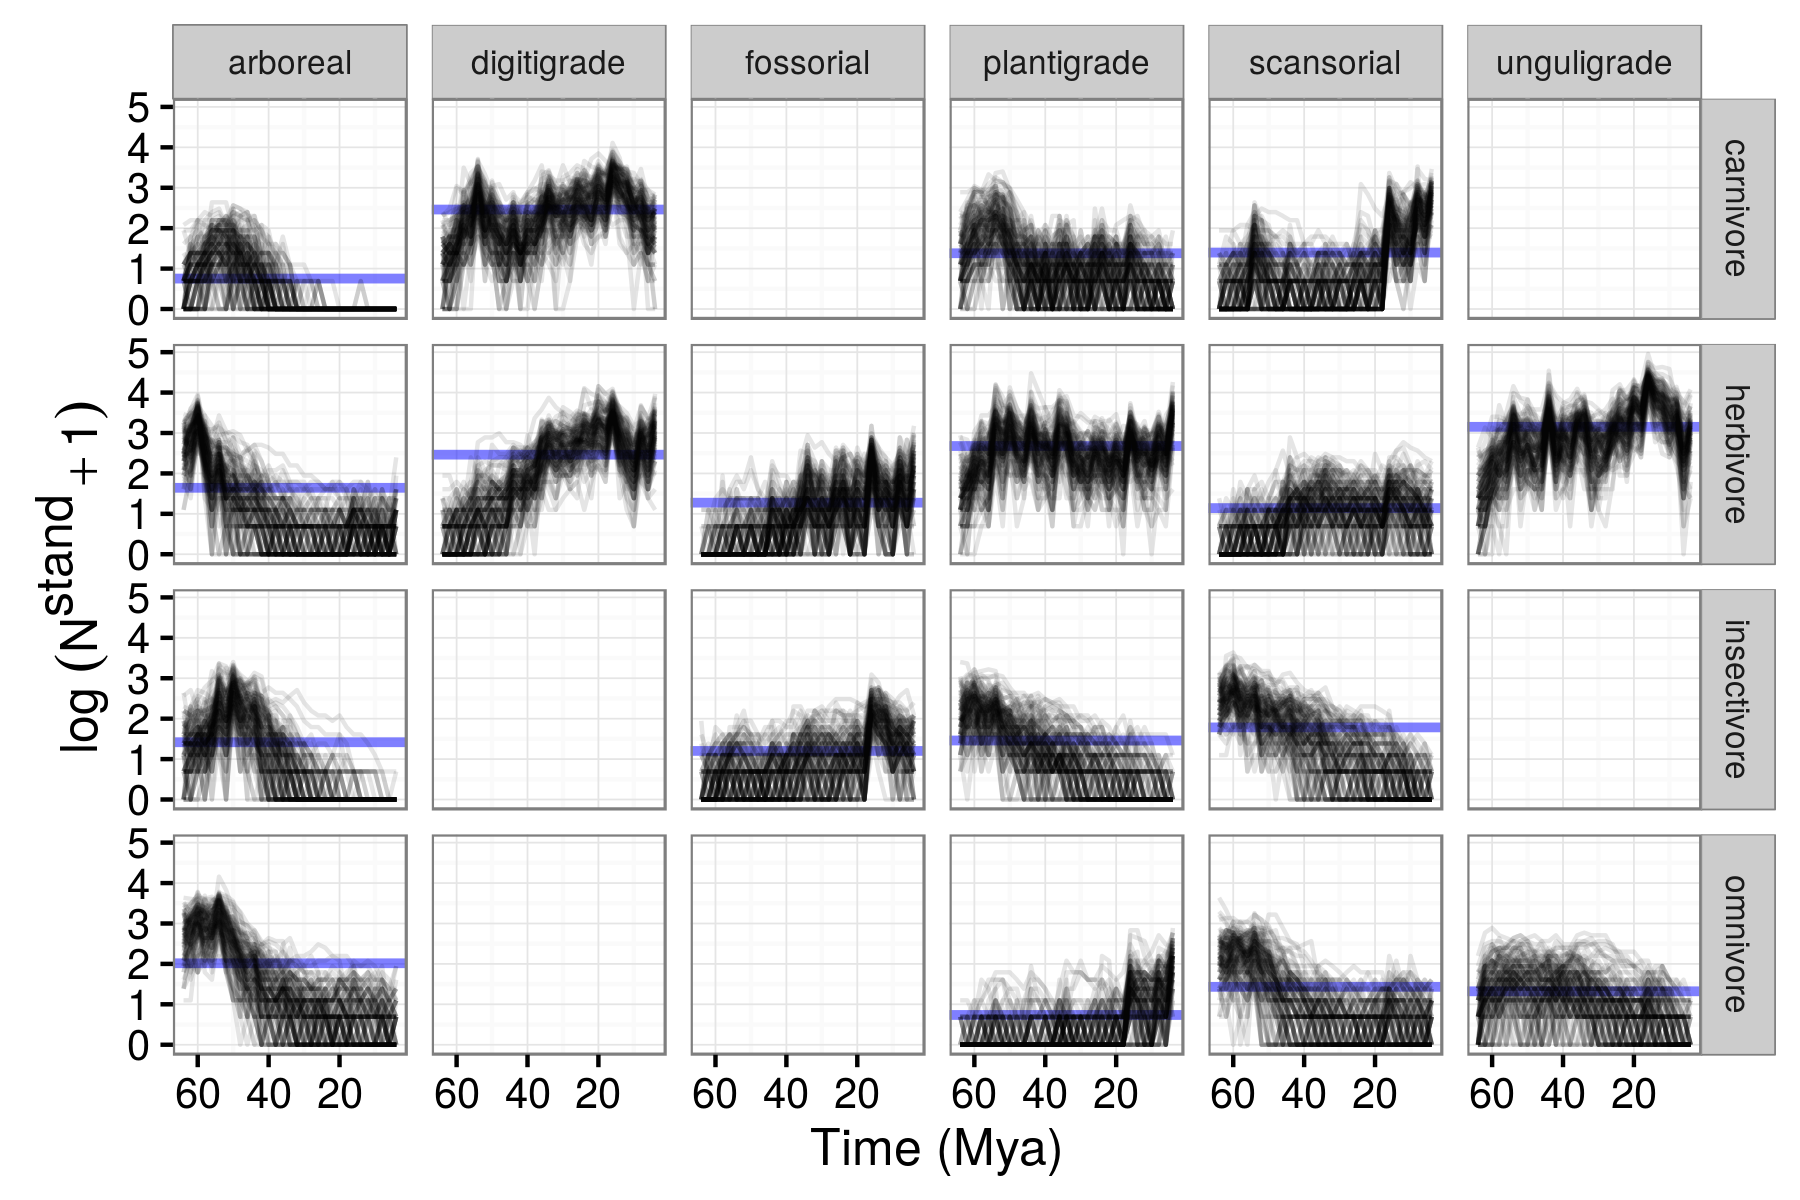
\includegraphics[width=\textwidth,height=0.4\textheight,keepaspectratio=true]{figure/ecotype_diversity}
  \caption[Estimated mammal ecotype log-diversity for the Cenozoic]{Posterior of standing log-diversity of North American mammals by ecotype for the Cenozoic as estimated from the birth-death model; 100 posterior draws are plotted to indicate the uncertainty in these estimates and what is technically plotted is log of diversity plus 1.}
  \label{fig:ecotype_diversity}
\end{figure}

Arboreal ecotypes obtain peak diversity early in the Cenozoic and then decline for the rest of the time series, becoming increasingly rare or absent as diversity approaches the Recent (Fig. \ref{fig:ecotype_diversity}). Arboreal herbivores and omnivores obtain peak diversity at the beginning of the Cenozoic then go into decline while remaining a small part of the species pool, while arboreal carnivores and insectivores obtain peak diversity 52-50 Mya and then quickly decline and become extremely rare or entirely absent from the species pool. This is consistent with increasing extinction risk in the Neogene compared to the Paleogene as proposed by \citet{Smits2015b}.

The diversity of digitigrade and unguligrade herbivores increases over the Cenozoic (Fig. \ref{fig:ecotype_diversity}). In contrast, plantigrade herbivore diversity does not have a single, broad-strokes pattern; instead, diversity increases, decreases, and may have then increased till the Recent. In contrast, fossorial and scansorial herbivores demonstrate a much flatter history of diversity, with a slight increase in diversity that over time is more pronounced among fossorial taxa than scansorial taxa. The expansion of digitigrade and unguligrade herbivores over the Cenozoic is consistent with the gradual expansion of grasslands which these ecotypes are better adapted to than closed environments \citep{Blois2009,Stromberg2005}.

Digitigrade carnivores have a multi-modal diversity history, with peaks at 54-52 and 12-10 Mya (Fig.\ref{fig:ecotype_diversity}). Between these two peaks digitigrade carnivore diversity dips below average diversity following the first peak and then grows slowly until the second peak. Plantigrade carnivores obtain peak diversity in the early Cenozoic and then maintain a relatively stable diversity until another peak at the end of the Cenozoic. The generally flat diversity history digitigrade carnivores lacks any sustained temporal trends and seems to reflect previous findings of limited diversity in spite of constant turnover and morphological evolution \citep{Valkenburgh1999,Silvestro2015b,Slater2015c}

There are some broad similarities in diversity histories of insectivorous and omnivorous taxa. The diversity histories of arboreal, plantigrade, and scansorial insectivorous taxa all demonstrate a decreasing pattern with time, while fossorial insectivores have a flat diversity history with a peak approximately 10 Mya (Fig. \ref{fig:ecotype_diversity}). Arboreal and scansorial omnivores decrease in diversity from their initial peaks early in the Cenozoic, and plantigrade omnivores have a generally flat diversity history with a sudden peak in diversity late in the Cenozoic (Fig. \ref{fig:ecotype_diversity}). Unguligrade omnivores also demonstrate a possible decrease in diversity over the Cenozoic, but not as clearly as arboreal and scansorial omnivores.


The waxing and waning of the mammal ecotypes is obvious when comparing changes to estimated relative log-mean of diversity (Fig. \ref{fig:ecotype_relative}). While ecotype diveristy does appear to change gradually, there are definite changes to the relative contributions of the ecotypes to the regional species pool. All arboreal ecotypes clearly decrease in relative diversity over the Cenozoic. In contrast the the digitigrade herbivore, fossorial herbivore, scansorial herbivore, and unguligrade herbivore ecotypes which increase in relative diversity over the Cenozoic. The digitigrade carnivore ecotype increases in relative diveristy until approximately the start of the Neogene, after which it maintains a generally constant relative diveristy; this is consistent with previous observations of constant or density-dependent diversity of the canid guild for the Neogene \citep{Valkenburgh1999,Silvestro2015b,Slater2015c}, a guild that overlaps with the digitigrade carnivore ecotype. Plantigrade herbivores remain a constant relative contribution to ecotypic diveristy. These results support the hypothesis of a gradual transition from the early Paleogene with a region with more avaliable habitat for aboreal taxa and less avaliable habitat for many digitigrade and unguligrade taxa, to an environment where arboreal taxa are absent from the species pool and digitigrade and unguligrade taxa are much more dominant (Fig. \ref{fig:ecotype_relative}). It is the relative contributions of digitgrade carnivores, digitigrade herbivores, and unguligrade herbivores which really shape the regional species pool of the Neogene. 


\begin{figure}[ht]
  \centering
  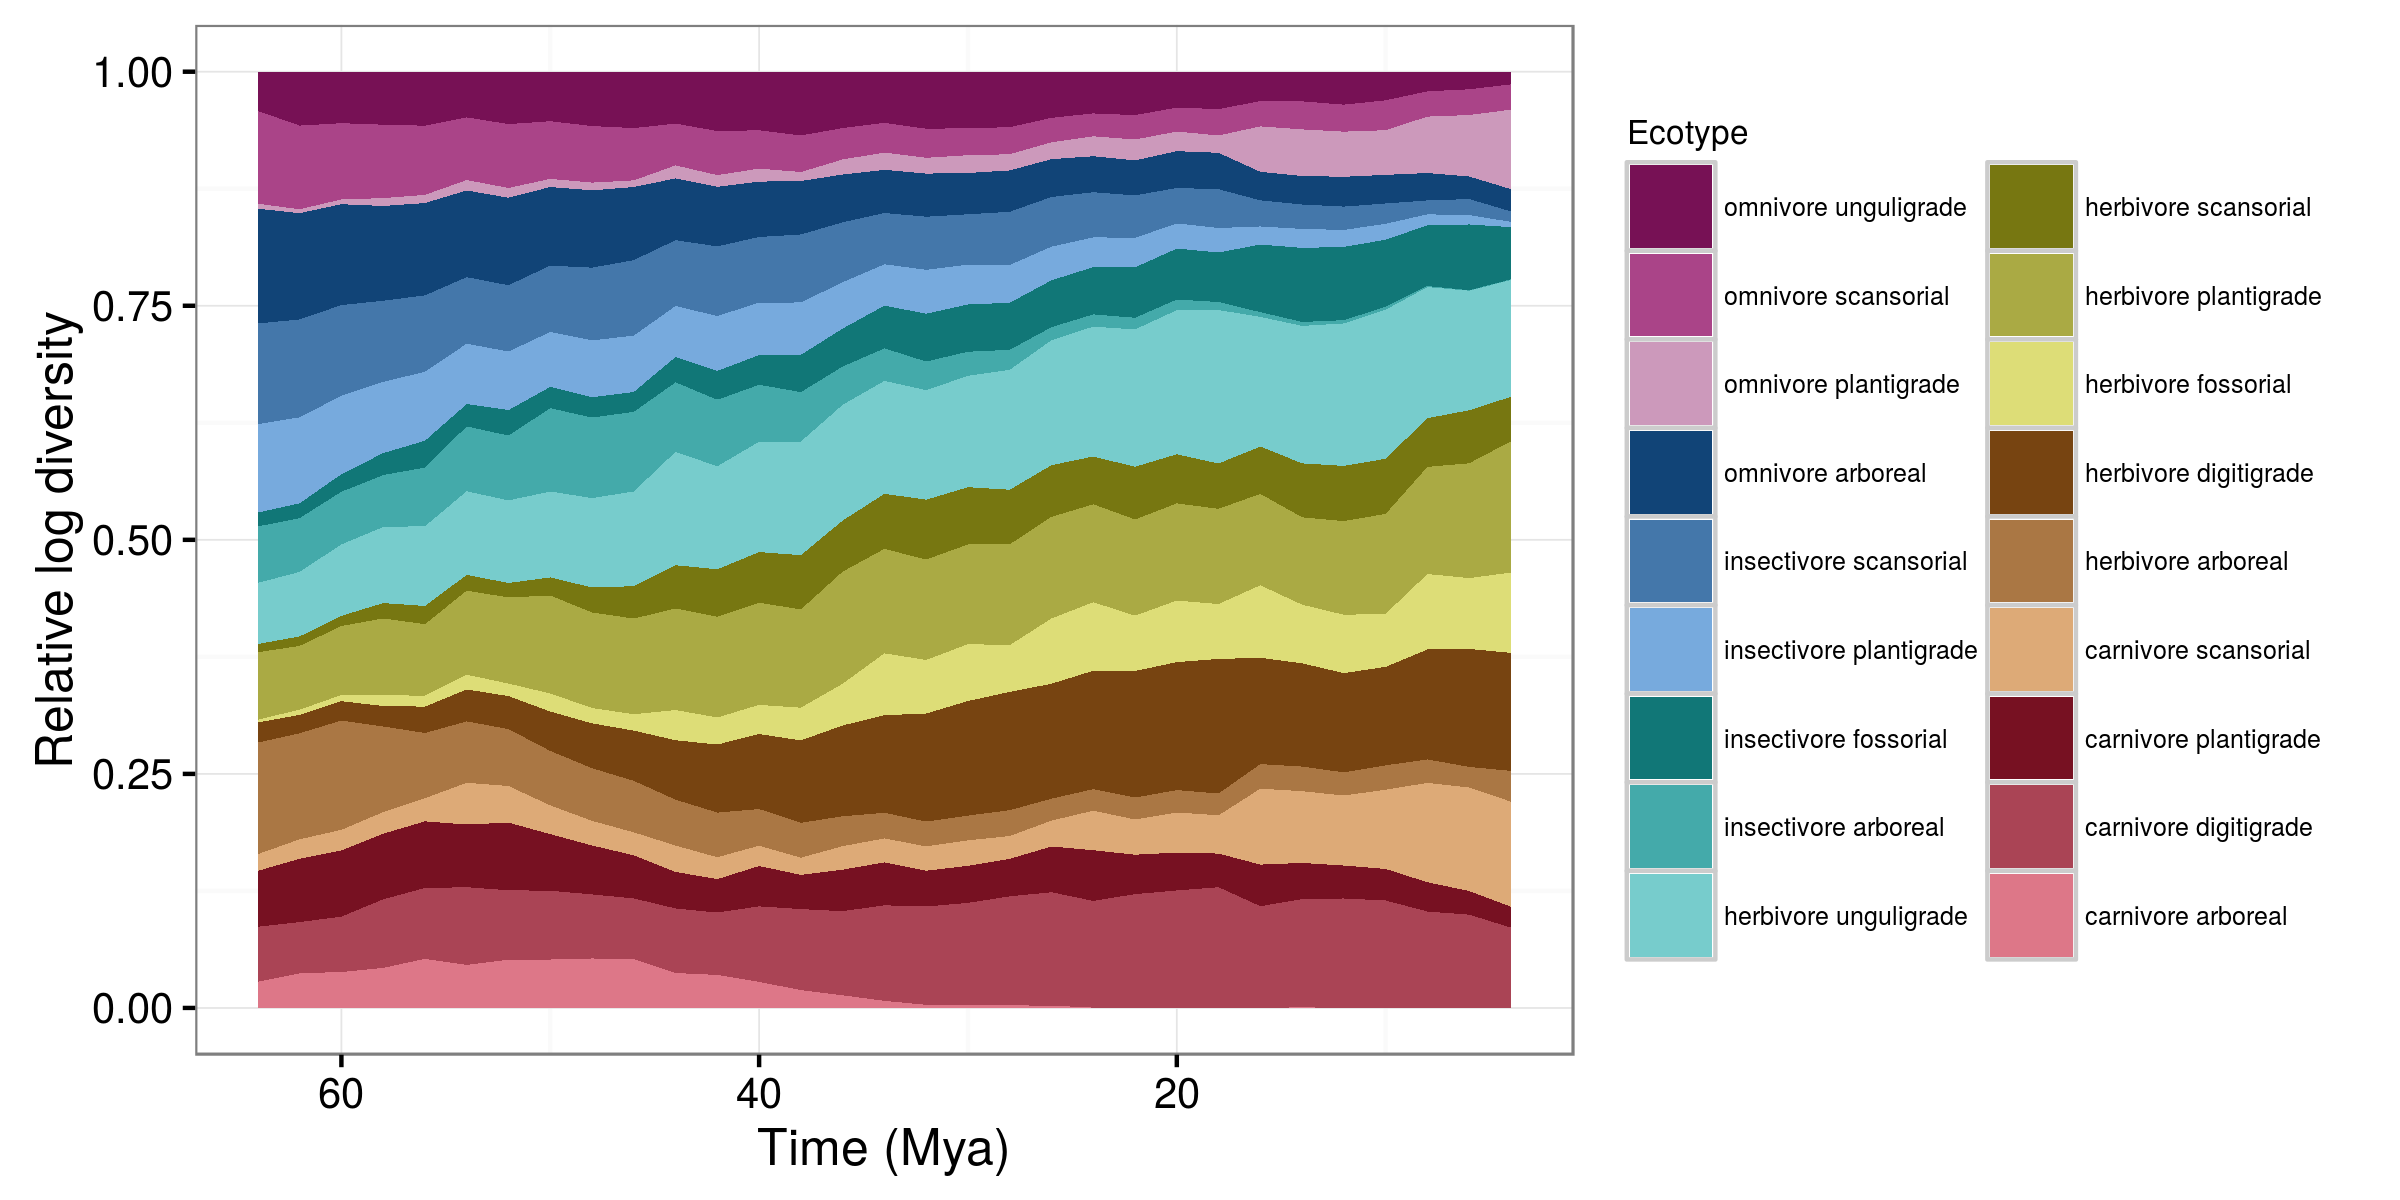
\includegraphics[width=\textwidth,height=0.4\textheight,keepaspectratio=true]{figure/relative_diversity}
  \caption[Relative mammal ecotype log-diversity for the Cenozoic]{Mean posterior estimate of relative log standing diveristy of 18 North American mammal ecotypes for the Cenozoic. These estimates are calculated from 100 posterior estimates of the true occurrence matrix \(z\) as estimated from the birth-death model.}
  \label{fig:ecotype_relative}
\end{figure}


Many of the estimated ecotype-specific diversity histories share a similar increase in diversity in the late Cenozoic, 16-14 Mya (Fig. \ref{fig:ecotype_diversity}). These increases are either sustained or temporary and are seen in digitigrade carnivores, plantigrade carnivores, scansorial carnivores, unguligrade herbivores, fossorial insectivores, and plantigrade omnivores.

When ecotype diversity is decomposed into per capita origination (Fig. \ref{fig:ecotype_birth}) and per capita extinction rates (Fig. \ref{fig:ecotype_death}) the way in which their diversity developed can be exampled. For ecotype-specific origination and extinction rates, the number of origination or extinction events for each ecotype was calculated and that number was divided by the total standing diversity of all mammals at the time. 

As should be expected, origination rates have a much greater range of values with a few very large spikes that line up with the spikes in over all diversification rate (Fig. \ref{fig:diversity_rate}). Importantly, the source of the massive increase in diversification rate at 16 Mya can be attributed almost solely to the origination of unguligrade herbivores (Fig. \ref{fig:ecotype_birth}). Additionally, by decomposing origination rate by ecotype, it is possible to identify a few possible cross-ecotype increases in origination rate. For example, digitigrade carnivores, digitigrade herbivores, and plantigrade herbivores share a lot of increases in origination rate with unguligrade herbivores; these are all ecotypes that demonstrate an obvious increase in diversity during the Paleogene and then maintain relatively high diversity through out the Neogene (Fig. \ref{fig:ecotype_diversity}).

In contrast to ecotype-specific per capita origination rates which demonstrate distinct peaks, the estimates of ecotype-specific per capita are more of a smear (Fig. \ref{fig:ecotype_death}). There are few increases in extinction rate that are shared across ecotypes. The per captia extinction rates of digitigrade, plantigrade, and unguligrade herbivores are lower in Paleogene than the Neogene. This result is interpreted to mean that as the diversity of these three ecotypes was increasing, the number of extinction events was also increasing. Also, the per capita extinction rate of arboreal taxa is higher in the Paleogene than the Neogene. While this result may seem odd considering the observed diversity pattern for these ecotypes (Fig. \ref{fig:ecotype_diversity}), I argue that this result is actually extremely intuitive: if there are no species of that ecotype originating or present, than there can be extinctions. This result highlights the distinction between extinction risk and extinction rate; an ecotype can have a high extinction risk, but if that ecotype is not present in the species pool in the first place than it has no associated extinction rate. 

\begin{figure}[ht]
  \centering
  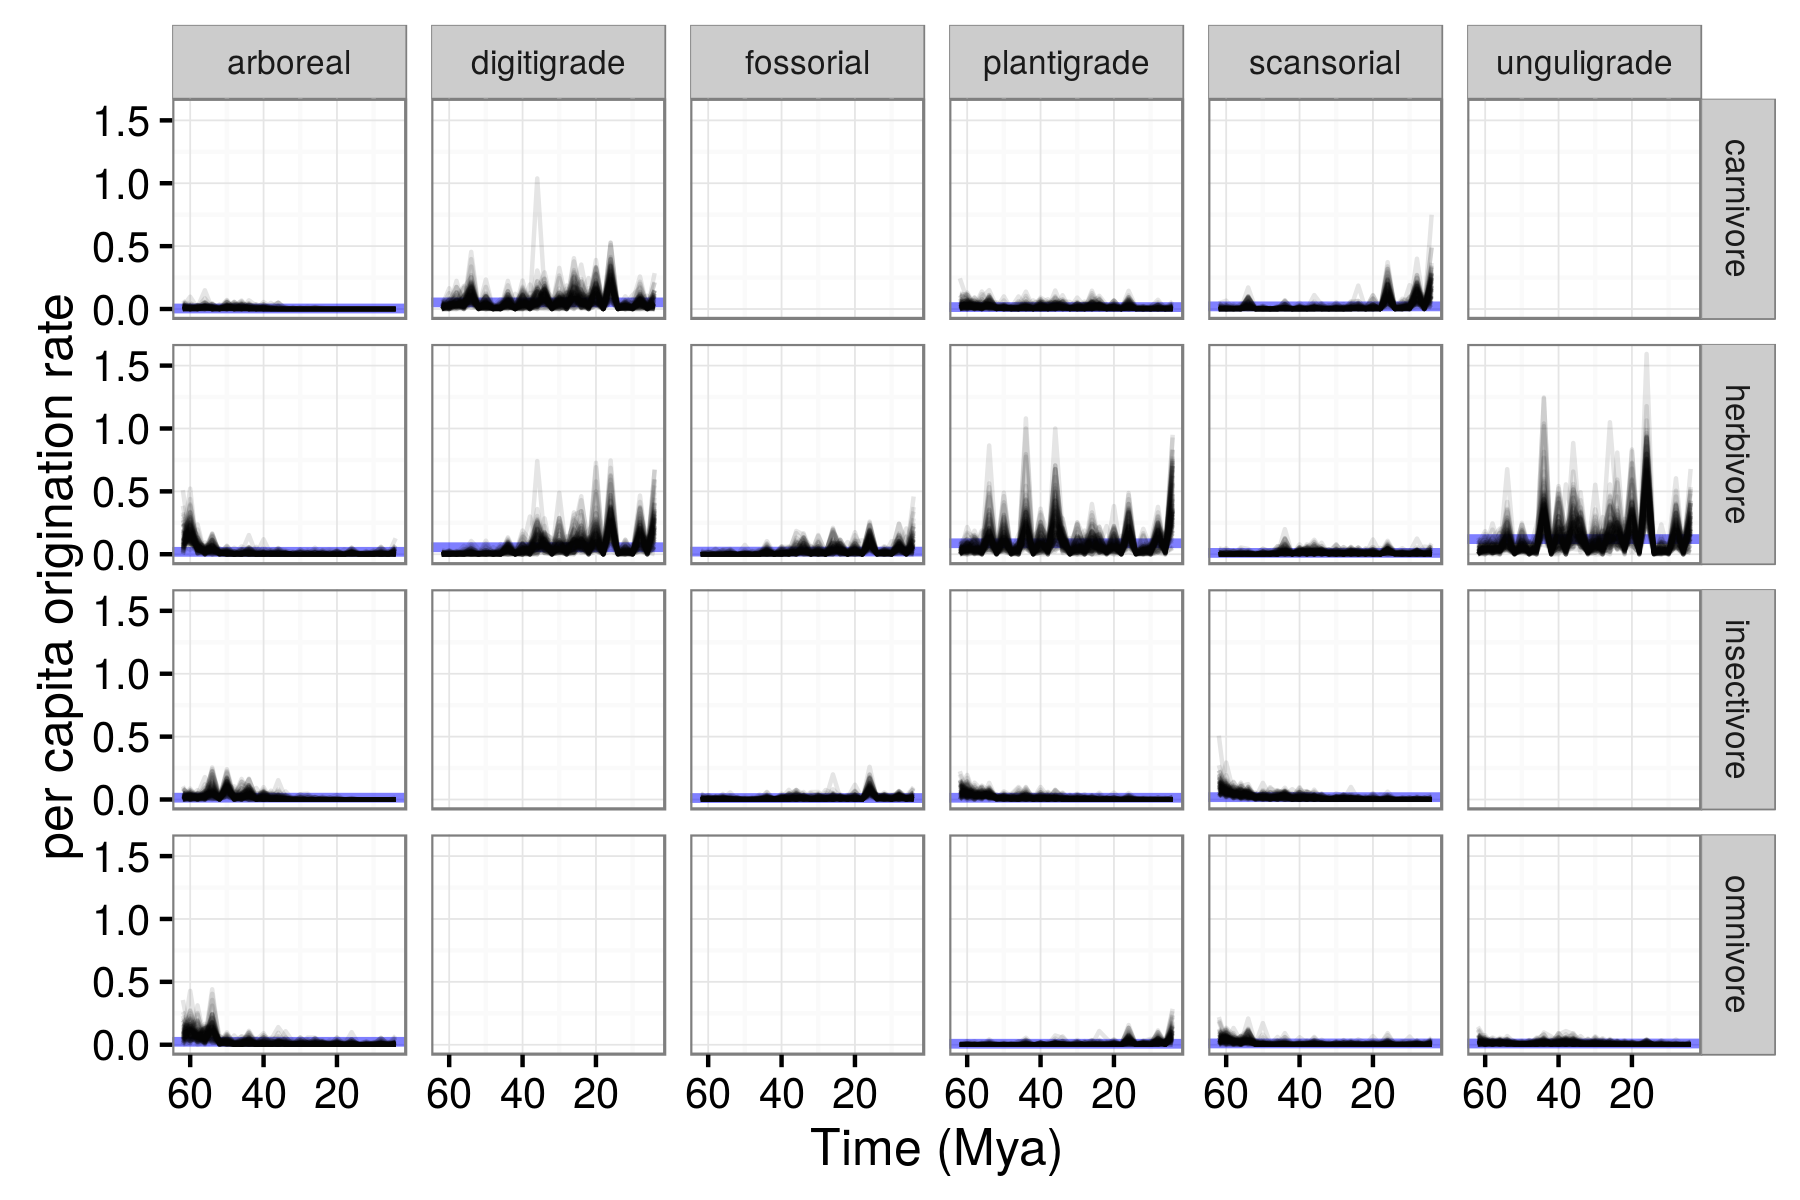
\includegraphics[width=\textwidth,height=0.4\textheight,keepaspectratio=true]{figure/birth_eco}
  \caption[Estimated per capita origination rates by mammal ecotype]{Posterior estimates of the per capita origination rates for each ecotype, plotted at the bin they originate from. These rates are calculated as the number of origination events for that ecotype from one time point to the next, divided by the standing diversity of all mammals at the initial time point. 100 posterior draws are plotted to indicate the uncertainty in these estimates.}
  \label{fig:ecotype_birth}
\end{figure}

\begin{figure}[ht]
  \centering
  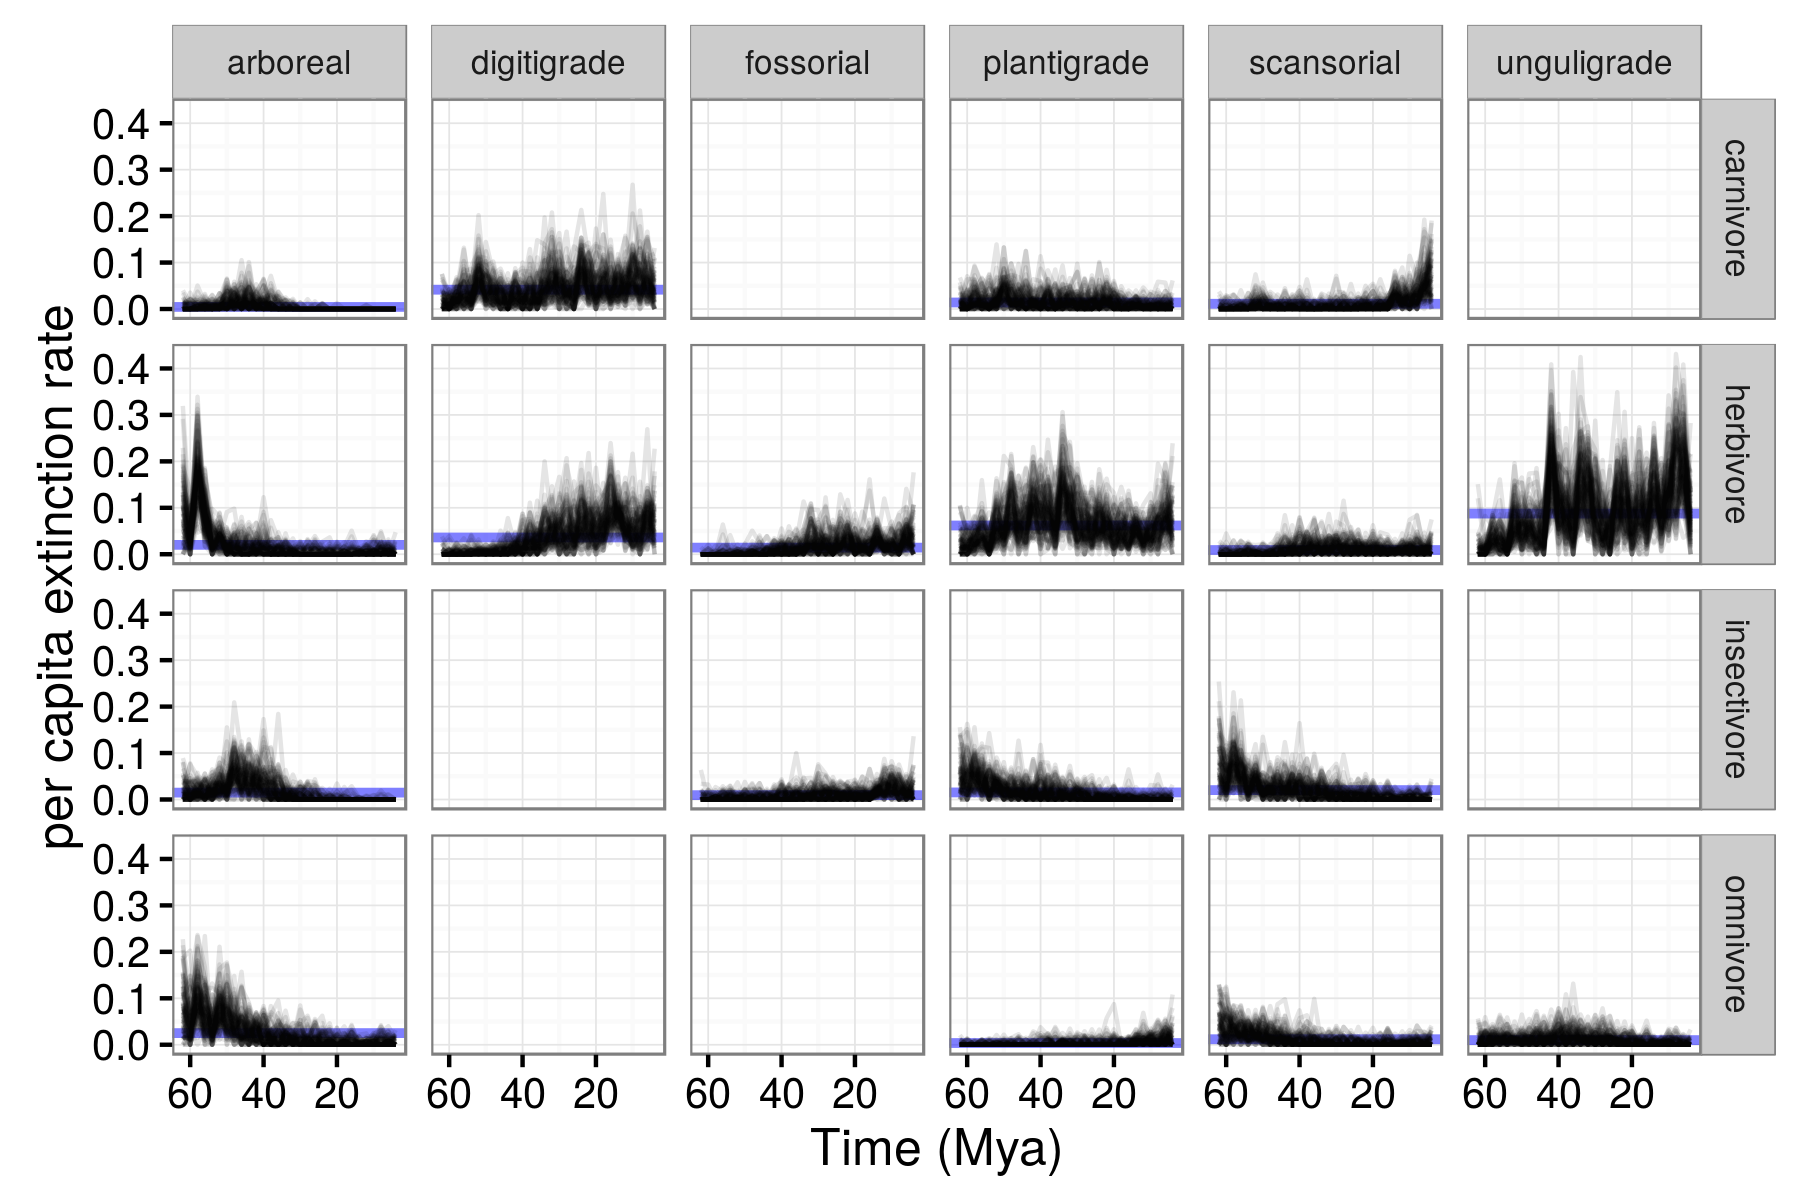
\includegraphics[width=\textwidth,height=0.4\textheight,keepaspectratio=true]{figure/death_eco}
  \caption[Estimated per capita extinction rates by mammal ecotype]{Posterior estimates of the per capita extinction rates for each ecotype, plotted at the bin they go extinct from. These rates are calculated as the number of extinction events for that ecotype from one time point to the next, divided by the standing diversity of all mammals at the initial time point. 100 posterior draws are plotted to indicate the uncertainty in these estimates.}
  \label{fig:ecotype_death}
\end{figure}


\end{document}

